\documentclass[11pt, a4paper, UKenglish, oneside]{book}

\usepackage[UKenglish]{babel}
\usepackage{BA_Titelseite}
\usepackage{tikz}

%Namen des Verfassers der Arbeit
\author{Giulia Liconti}
%Geburtsdatum des Verfassers
\geburtsdatum{21. November 2004}
%Gebortsort des Verfassers
\geburtsort{Bologna}
%Datum der Abgabe der Arbeit
\date{\today}

%Name des Betreuers
% z.B.: Prof. Dr. Peter Koepke
\betreuer{Advisor: Prof. Dr. Margerita Disertori}
%Name des Zweitgutachters
\zweitgutachter{Second advisor: Dr. Davide Macera}
%Name des Instituts an dem der Betreuer der Arbeit tätig ist.
%z.B.: Mathematisches Institut
\institut{Institut of applied Mathematics}
%\institut{Mathematisches Institut}
%\institut{Institut f\"ur Angewandte Mathematik}
%\institut{Institut f\"ur Numerische Simulation}
%\institut{Forschungsinstitut f\"ur Diskrete Mathematik}
%Titel der Bachelorarbeit
\title{Self-avoiding walks in Anderson localization}
%Do not change!
\ausarbeitungstyp{Bachelor's Thesis Mathematics}

\usepackage{amsmath}
\usepackage{amssymb}
\usepackage{amsthm}
\usepackage[alphabetic]{amsrefs}

\theoremstyle{plain}
\newtheorem{theorem}{Theorem}
\newtheorem{proposition}[theorem]{Proposition}
\newtheorem{lemma}[theorem]{Lemma}
\newtheorem{corollary}[theorem]{Corollary}
\theoremstyle{remark}
\newtheorem{remark}[theorem]{Remark}
\newtheorem{note}[theorem]{Note}
\theoremstyle{definition}
\newtheorem{definition}[theorem]{Definition}
\numberwithin{equation}{section}
\numberwithin{theorem}{section}
\newtheorem{claim}[theorem]{Claim}
\newtheorem{example}[theorem]{Example}


\usepackage{mathtools}
\DeclarePairedDelimiter\abs{\lvert}{\rvert}
\DeclarePairedDelimiter\norm{\lVert}{\rVert}

\usepackage[T1]{fontenc}
\usepackage[utf8]{inputenc}
\usepackage[hidelinks]{hyperref}
\usepackage{setspace}
\usepackage{graphicx}
\usepackage{xcolor}

\begin{document}
\setstretch{1.15}
\maketitle


\clearpage
\tableofcontents
\newpage

\clearpage
\addcontentsline{toc}{chapter}{Introduction}
\chapter*{Introduction}
The Anderson localization model was introduced by the physicist P.W. Anderson in 1958 \cite{anderson1958} to explain the quantum mechanical effects of disorder in materials.
In particular, Anderson's purpouse was to study the behavior of electrons in a lattice with disordered potential energy on the sites, which is the quantum mechanical analogue of a random walk in a random environment.\\

The model is governed by a random Schr\"odinger operator that describes the total energy of the system. This operator is composed of a kinetic term and a random potential term. The kinetic energy allows the particles to hop from site to site, while the random potential disturbs their motion through the material.
When the disorder is sufficiently strong, these particles become trapped in a localized region and can no longer spread to conduct electricity. This phenomenon is known as Anderson localization, and it effectively turns the material into an insulator. 
This stands in sharp contrast to the behavior of electrons in ideal, perfectly ordered crystals, which naturally act as conductors.\\

In the last decades, the study of random operators has become an important field of mathematical physics.
The two important methods that have been used to prove on which condition on the disorder level Anderson localization holds are the \textit{multiscale analysis} (MSA), developed by Fr\"ohlich and Spencer \cite{frohlich1983}, and the 
\textit{ fractional moment method} (FMM) by Aizenman and Molchanov \cite{aizenman1993}. The multiscale analysis method focuses on the bound of the second moments of the operator's resolvent, whereas the fractional moments method utilizes its fractional powers. In this thesis, we are going to focus on the second one, combined wit the self-avoiding-walks method. 
\subsection*{Structure of the thesis}
In Chapter 1, we introduce the Anderson model, more spacifically we will distinguish two variations of it: the nearest-sites model and the long-range model. focusing on the properties of its components, its spectrum, and the main results of this thesis.\\

\noindent
In Chapter 2, we define spectral and dynamical localization. We also define exponential dynamical localization and show how it implies that all moments of the position operator remain bounded in time.\\

\noindent
In Chapter 3, we introduce the Green function as the resolvent of the model and explore how the exponential decay of its fractional power leads to localization. Specifically, we also introduce two central analytical tools, such as the \textit{resolvent identity} of linear operators and the resulting \textit{a priori bound}.\\

\noindent
In Chapter 4, we provide the preliminary definitions for self-avoiding walk (SAW) methods and obtain the main results of this thesis using a new representation for the Green function. We will focus on both exponential decay for the standard model, and polinomial decay for the fractional model. \\

\noindent
Finally,  Chapter 5 is dedicated to the open problems concering th evalues of the disorder parameter in different dimensions.


\clearpage
\chapter{The Anderson Model}
In this chapter, the random Schr\"odinger operator is the center of our attention. First, we define it as the \textit{Hamiltonian} and discuss the physical meaning of its time-evolving solutions. We are going to define two variation of this model: the standard Anderson model, with near-neighbors jumps, and the fractional Anderson model, with long-range jumps. Right after, we focus on the properties of each of their components and their spectra. Finally, we discuss the main results.\\
\section{The Hamiltonian}
\label{sec:The_Hamiltonian}
Transport phenomena in disordered materials are often described via discrete random Schr\"odinger operators. In quantum mechanics, the \textit{Hamiltonian} represents the total energy of the system, decomposing naturally into kinetic and potential energy. It takes the form of an infinite random matrix on the lattice $\mathbb{Z}^d$, 
\begin{equation}
    H_{\omega,\alpha} = (- \Delta)^\alpha + \lambda V_\omega,
\end{equation}
where $(-\Delta)^{\alpha}$ is a deterministic matrix representing the kinetic energy, $V_\omega$ is a diagonal matrix with random entries representing the disordered potential, and $\lambda$ is the disorder parameter.\\
For $\alpha=1$, the kinetic energy is defined by the standard discrete laplacian, which lets the particles jump from one site to the first-neighbors.\\
For $\alpha <1$, the kinetic energy is defined by the fractional discrete laplacian, which provides jumps of any arbitrary distance in the grid.\\
This operator acts on the Hilbert space of square summable sequences
\[
\ell^2(\mathbb{Z}^d) = \left\{ u : \mathbb{Z}^d \to \mathbb{C} \ \middle| \ \sum_{x \in \mathbb{Z}^d} |u(x)|^2 < \infty \right\}
\]
with the inner product defined as $\langle u, v \rangle = \sum_{x \in \mathbb{Z}^d} \overline{u(x)} v(x)$.\\

The mathematical space $\ell^2(\mathbb{Z}^d)$ is exactly where the physical reality of the electron is recorded. In quantum mechanics, the state of the system is described by a vector in this space : a normalized wave function $\psi \in \ell^2(\mathbb{Z}^d)$, such that
\[
\|\psi\|_{\ell^2}^2 = \sum_{x \in \mathbb{Z}^d} |\psi(x)|^2 = 1.
\]
The quantity $P(x) = |\psi(x)|^2$ defines a probability mass function on the lattice $\mathbb{Z}^d$, representing the exact probability of finding the particle at site $x$. 

The state functions are the solutions to the time-dependent Schr\"odinger equation $H_\omega \psi(t) = i\partial_t \psi(t)$. Because the resulting time evolution operator $e^{-itH_\omega}$ is unitary on $\ell^2(\mathbb{Z}^d)$, the total probability is conserved at all times $t \in \mathbb{R}$:
\begin{equation}
\|\psi(t)\|_{\ell^2}^2 = \|e^{-itH_\omega}\psi_0\|_{\ell^2}^2 = \|\psi_0\|_{\ell^2}^2 = 1.
\end{equation}

In particular, if the particle is initially placed at a specific site $x \in \mathbb{Z}^d$ with $\psi_0 = \delta_x$, the transition probability to find the particle at site $y \in \mathbb{Z}^d$ at time $t$ is given by the squared transition amplitude:
\begin{equation}
P(x \to y; t) = |\langle \delta_y, e^{-itH_\omega} \delta_x \rangle|^2.
\end{equation}

As we will see later, under certain conditions on the disorder parameter, this probability $P$ tends to $0$ at all times $t$ as the distance $|x-y| \to \infty$, mathematically proving that the particle remains trapped. In particular, the decay changes from exponential to polinomial, as $\alpha =1$ or $\alpha \in (0,1)$.
\vspace{0.3 cm}

\subsection*{The  Discrete Laplacian}
The  discrete Laplacian is the  discrete analogue of the usual Laplacian ($ \sum_j \partial^2/\partial x_j^2$). First, we consider the properties of this operator for $\alpha=1$ and then we compare the fractional case, for $\alpha \in (0,1)$.
\subsection*{$\boldsymbol{(- \Delta)^{\alpha}}$ for $\boldsymbol{\alpha =1}$}
For the functions $u \in \ell^2(\mathbb{Z}^d)$ it is defined as

\begin{equation}
    -\Delta u(x) := \sum_{y \in \mathbb{Z}^d,|x-y|=1} u(x) - u(y) \quad \text{for } x \in \mathbb{Z}^d.
\end{equation}
where $|*|$ denotes the euclidean norm.

For each site $x$, there are $2d$ possible $y$ such that $|x-y|=1$. Thus, we can define an infinte matrix such that \[
(-\Delta)(x,y) = \begin{cases} 
2d & \text{if } x = y  \\
-1 & \text{if } |x - y| = 1  \\
0 & \text{otherwise}
\end{cases}
\]

The discrete Laplacian represents the kinetic term and connects neighboring sites on the lattice, allowing the electron to transition from one to another.

The operator $-\Delta$ is bounded and self-adjoint on $\ell^2(\mathbb{Z}^d)$. To establish boundedness , we verify \textbf{summability} for any $u \in \ell^2(\mathbb{Z}^d)$. We can show this through the following,
\begin{align*}
\sum_{x \in \mathbb{Z}^d} |-\Delta u(x)|^2 &= \sum_{x \in \mathbb{Z}^d} | \sum_{\substack{y \in \mathbb{Z}^d \\ |x - y| = 1}} \bigl(u(x) - u(y)\bigr)|^2 \\
&\leq  \sum_{x \in \mathbb{Z}^d} \left(2d \sum_{|x - y| = 1} |u(x) - u(y)|^2 \right) \\
&\leq 2d \sum_{x \in \mathbb{Z}^d} \left( \sum_{|x - y| = 1} \left(|u(x)|^2 + |u(y)|^2+2|u(x)u(y)|\right) \right) \\
&\leq 2d \sum_{x \in \mathbb{Z}^d} \left( 2 \sum_{|x - y| = 1} \left(|u(x)|^2 + |u(y)|^2\right) \right) \\
&= 2d \cdot 2 \cdot 4d \|u\|_{\ell^2}^2 = 16d^2 \|u\|_{\ell^2}^2 < \infty,
\end{align*}
where we applied the Cauchy-Schwarz inequality to the sum over the $2d$ neighbors, followed by Young's inequality, and finally the translation invariance of the $\ell^2$ norm. 
This guarantees the operator is \textbf{bounded}, since
\[
\frac{\|-\Delta u\|_{\ell^2}^2}{\|u\|_{\ell^2}^2} \le 16 d^2 \implies \|-\Delta\| = \sup_{u \ne 0} \frac{\|-\Delta u\|_{\ell^2}}{\|u\|_{\ell^2}} \le 4d.
\]

To prove \textbf{self-adjointness} for a bounded operator, we only need to show symmetry. For $u, v \in \ell^2(\mathbb{Z}^d)$:
\begin{align*}
\langle u, -\Delta v \rangle &= \sum_{x \in \mathbb{Z}^d} \overline{u(x)} \left( \sum_{|x - y| = 1} (v(x) - v(y)) \right) \\
&= \sum_{x \in \mathbb{Z}^d} \left( 2d \overline{u(x)} v(x) -  \sum_{|x - y| = 1} \overline{u(x)} v(y)\right)\\
&=\sum_{x \in \mathbb{Z}^d} 2d \overline{u(x)} v(x) - \sum_{x \in \mathbb{Z}^d} \sum_{|x - y| = 1} \overline{u(y)} v(x) \\
&= \sum_{x \in \mathbb{Z}^d} v(x) \left( \sum_{|x - y| = 1} (\overline{u(x)} - \overline{u(y)}) \right)\\
 &= \sum_{x \in \mathbb{Z}^d} v(x) \overline{(-\Delta u(x))} = \langle - \Delta u, v \rangle.
\end{align*}
\vspace{1em}

The spectrum of a bounded, self-adjoint operator is a compact subset of $\mathbb{R}$, which in this case is exactly the closed interval $[0,4d]$. This range represents the allowed kinetic energy levels an electron can possess. 

To understand this result explicitly, we apply the discrete Fourier transform:
\[
\mathcal{F} \colon \ell^2(\mathbb{Z}^d) \longrightarrow L^2([0, 2\pi)^d)
\]
defined by
\[
(\mathcal{F}u)(k) \coloneqq \lim_{N \rightarrow \infty} (2\pi)^{-\frac{d}{2}} \sum_{|x| \leq N} u(x)\, e^{- i k \cdot x}, \qquad k \in [0, 2\pi)^d.
\]

We first assume $u \in \ell^1(\mathbb{Z}^d)$. Because $\ell^1(\mathbb{Z}^d)$ is a dense subset of $\ell^2(\mathbb{Z}^d)$ and the Fourier transform $\mathcal{F}$ is unitary, we can extend the results by continuity to all functions in $\ell^2(\mathbb{Z}^d)$.
\begin{align*}
    (\mathcal{F} (-\Delta u))(k) &= (2\pi)^{-\frac{d}{2}} \sum_{x \in \mathbb{Z}^d} (-\Delta u)(x)\, e^{-i k \cdot x} \\
    &= (2\pi)^{-\frac{d}{2}} \sum_{x \in \mathbb{Z}^d} \left( \sum_{|y-x|=1} \bigl(u(x) - u(y)\bigr) \right) e^{-i k \cdot x} \\
    &= (2\pi)^{-\frac{d}{2}} \sum_{x \in \mathbb{Z}^d} \left( 2d\, u(x) - \sum_{|y-x|=1} u(y) \right) e^{-i k \cdot x} \\
    &= 2d\,(\mathcal{F}u)(k) - (2\pi)^{-\frac{d}{2}} \sum_{x \in \mathbb{Z}^d} \sum_{|y-x|=1} u(y)\, e^{-i k \cdot x} \\
    &= 2d\,(\mathcal{F}u)(k) - (2\pi)^{-\frac{d}{2}} \sum_{y \in \mathbb{Z}^d} u(y) \sum_{|m|=1} e^{-i k \cdot (y+m)} \quad \text{\small (setting $m = x - y$)} \\
    &= 2d\,(\mathcal{F}u)(k) - \left( (2\pi)^{-\frac{d}{2}} \sum_{y \in \mathbb{Z}^d} u(y)\, e^{-i k \cdot y} \right) \sum_{|m|=1} e^{-i k \cdot m} \\
    &= 2d\,(\mathcal{F}u)(k) - (\mathcal{F}u)(k) \sum_{j=1}^d \left( e^{-i k_j} + e^{i k_j} \right) \\
    &= \left( 2 \sum_{j=1}^d ( 1-\cos(k_j)) \right)  (\mathcal{F}u)(k).
\end{align*}
Thus, the Laplacian acts as a simple multiplication operator in Fourier space
$$ \mathcal{F} (-\Delta) \mathcal{F}^{-1} =  2 \sum_{j=1}^d (1-\cos(k_j)) $$ 
on $L^2([0,2\pi)^d)$ in the momentum variable $k= (k_1,\dots, k_d)$. 

\begin{remark}
    The discrete Laplacian has no true eigenvalues in $\ell^2(\mathbb{Z}^d)$. However, similar to the continuum Laplacian, it possesses plane waves as generalized eigenfunctions. For a fixed momentum $k \in [0,2\pi)^d$, we define:
    \[
    \phi_k(x) := e^{-i x \cdot k}.
    \]
    While $\phi_k \notin \ell^2(\mathbb{Z}^d)$ because it is not square-summable, the operator $(-\Delta)$ acts on it as
    \begin{align*}
        (-\Delta \phi_k)(x) &= \sum_{|m|=1} (e^{-ix \cdot k} - e^{-i(x+m)\cdot k}) \\
        &=  2d \phi_k(x) - \left( \sum_{j=1}^d 2\cos(k_j) \right) \phi_k(x) \\
        &= \left( 2 \sum_{j=1}^d (1-\cos(k_j)) \right) \phi_k(x).
    \end{align*}
    Thus, $\phi_k$ is a bounded, generalized eigenfunction of $(-\Delta)$ corresponding to the spectral value $2\sum_{j=1}^d (1-\cos(k_j))$. Since $\cos(k_j)$ oscillates between $-1$ and $1$, the spectrum of the discrete Laplacian is purely continuous and strictly bounded within the interval $[0,4d]$.
\end{remark}

\subsection*{$\boldsymbol{(- \Delta)^{\alpha}}$ for $\boldsymbol{0<\alpha<1}$}

The fractional kinetic operator is formally defined via the discrete Fourier transform by raising to a fractional power: 
\[
\mathcal{F} (-\Delta)^\alpha \mathcal{F}^{-1} = \left( 2 \sum_{j=1}^d ( 1-\cos(k_j)) \right)^{\alpha}.
\]
Like the standard discrete Laplacian, $(-\Delta)^\alpha$ is bounded, self-adjoint, and translation-invariant. 

However, its behavior in position space is fundamentally different. Instead of only connecting nearest neighbors, the fractional operator connects arbitrarily distant sites. Consequently, for any $x \ne y$, the matrix elements $(-\Delta)^\alpha(x,y)$ are strictly negative and never exactly zero. Instead, they exhibit a polynomial decay. There exist strictly positive constants $0 < c_{\alpha,d} \le C_{\alpha,d} < \infty$ such that:
\begin{equation}
\frac{c_{\alpha,d}}{|x-y|^{d+2\alpha}} \le -(-\Delta)^{\alpha}(x,y) \le \frac{C_{\alpha,d}}{|x-y|^{d+2\alpha}} \quad \forall x \ne y. \label{eq:fractionalbound}
\end{equation}

Because $d+2\alpha > d$ for any $\alpha \in (0,1)$, this polynomial decay ensures that the off-diagonal kernel is absolutely \textbf{summable}:
\begin{equation}
    \sum_{y \ne x \in \mathbb{Z}^{d}} |(-\Delta)^{\alpha}(x,y)| \le C_{\alpha,d} \sum_{y \ne x \in \mathbb{Z}^{d}} \frac{1}{|x-y|^{d+2\alpha}} < \infty. \label{eq: summabilityfrackernel}
\end{equation} 

This summability is crucial because it guarantees that the diagonal entries are strictly positive, well-defined, and finite:
\begin{equation}
    (-\Delta)^{\alpha}(x,x) = -\sum_{y\ne x}(-\Delta)^{\alpha}(x,y) > 0 \quad \forall x \in \mathbb{Z}^d. \label{eq:118}
\end{equation}

\begin{remark}
    The diagonal relation \eqref{eq:118} is the direct fractional analogue of the standard discrete Laplacian, where we had $(-\Delta)(x,x) = - \sum_{|x-y|=1} (-1) = 2d$. The critical distinction is that the standard Laplacian computes this value by summing over exactly $2d$ nearest neighbors. In the fractional case, because the particle can jump to any site, we sum over the entire lattice.
\end{remark}

We can already prove the summability of the fractional kernel too:
\begin{lemma}
    For any $\alpha \in (0,1)$ and $s \in \left(\frac{d}{d+2\alpha},1\right]$,
    \begin{equation}
    \sum_{x \in \mathbb{Z}^{d}} |(-\Delta)^{\alpha} (0,x)|^s < \infty \label{eq:Dsbound}
\end{equation}
\end{lemma}

\begin{proof}
From \eqref{eq:fractionalbound}:
$$ \sum_{|x| \ge 1, \, x \in \mathbb{Z}^d} |(-\Delta)^\alpha(0,x)|^s \le C_{\alpha,d}^s \sum_{|x| \ge 1, \, x \in \mathbb{Z}^d} \frac{1}{|x|^{(d+2\alpha)s}}.$$

By standard comparison of the lattice sum with an integral on $\mathbb{R}^d$:
\[
\sum_{|x| \ge 1, \, x \in \mathbb{Z}^d} \frac{1}{|x|^p} \le C_d \int_{|z|>1} \frac{1}{|z|^p} \, dz.
\]

Passing to spherical coordinates in $\mathbb{R}^d$, the integral reads
\begin{align*}
\int_{|z| > 1} \frac{1}{|z|^p} \, dz
&= |\mathbb{S}^{d-1}| \int_{1}^\infty \frac{r^{d-1}}{r^p} \, dr \\
&= |\mathbb{S}^{d-1}| \int_{1}^\infty r^{d - 1 - p} \, dr,
\end{align*}
where $|\mathbb{S}^{d-1}| = \frac{2\pi^{d/2}}{\Gamma(d/2)}$ denotes the surface area of the unit sphere in $\mathbb{R}^d$.

The radial integral converges if and only if the power satisfies
\[
d - 1 - p < -1 \iff p > d.
\]
Substituting $p = s(d+2\alpha)$, this condition becomes
\[
s(d + 2\alpha) > d \iff s > \frac{d}{d + 2\alpha}.
\]
Since $\alpha > 0$ implies $d + 2\alpha > d$; for every $s \in \left(\frac{d}{d+2\alpha}, 1\right]$, we conclude that
\[
\sum_{x \ne 0} |(-\Delta)^\alpha_{0,x}|^s \le C_{\alpha,d}^s \sum_{x \ne 0} \frac{1}{|x|^{s(d+2\alpha)}} < \infty.
\]
\end{proof}

\subsection*{The Random Potential}
The random potential is expressed as the multiplication operator $V_\omega(x)= \omega_x$. It is a diagonal matrix, where $ \omega = (\omega_x)_{x \in \mathbb{Z}^d}$ is a set of indipendent identically distributed real-valued random entries. Physically, $V_\omega$ represents the random electric potential created by nuclei at the sites $x \in \mathbb{Z}^d$.
\begin{figure}[ht!]
    \centering
    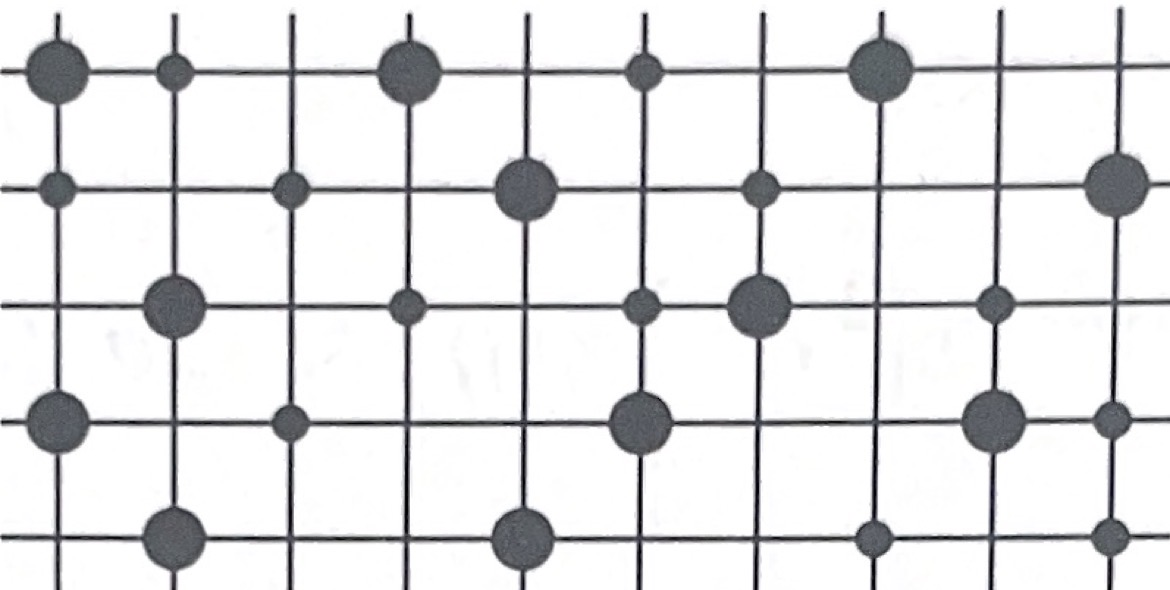
\includegraphics[width=0.4\textwidth]{IMG_1129.jpeg}
    \caption{A disordered lattice system. Picture from \cite{aizenman2015}}
\end{figure}

\begin{definition}[i.i.d. random variables]Let $(\Omega, \mathcal{A}, \mathbb{P})$ be a general probability space. A family of random variables $(\omega_x)_{x \in \mathbb{Z}^d}$ defined on $(\Omega, \mathcal{A}, \mathbb{P})$ is \textbf{identically distributed} if there exists a Borel probability measure $\mu$ on $\mathbb{R}$ such that $\mathbb{P}(\omega_x \in A) = \mu(A)$ for all $x \in \mathbb{Z}^d$ and all Borel sets $A \subset \mathbb{R}$.\\
The family $(\omega_x)_{x \in \mathbb{Z}^d}$ is \textbf{independent} if$$\mathbb{P}(\omega_{x_1} \in A_1, \dots, \omega_{x_l} \in A_l) = \prod_{j=1}^l \mathbb{P}(\omega_{x_j} \in A_j) = \prod_{j=1}^l \mu(A_j)$$for every finite subset of distinct indices $\{x_1, \dots, x_l\} \subset \mathbb{Z}^d$ and arbitrary Borel sets $A_1, \dots, A_l \subset \mathbb{R}$.
\end{definition}

In this thesis we assume that $\omega_x$ are uniformly distributed in the real closed interval $ [-1,1]$.\\
We consider then the probability space as the following infinite prduct space
\[
(\Omega, \mathcal{A},\mathbb{P})= \bigotimes_{x \in \mathbb{Z}^d} ([-1,1], \mathcal{B}([-1,1]), \mu),
\]
where $\mathcal{B}([-1,1])$ is the Borel $\sigma$-algebra and $ d\mu(\omega_x)= \rho(\omega_x)d\omega_x$ where the continuous density is given by $\rho= \frac{1}{2}\chi_{[-1,1]}$.
\begin{remark}
     It is possible to generalise the results to all absolutely continuous distributions where $\rho$ has compact support.
\end{remark}
   



As a diagonal operator, the spectrum of $V_\omega$ consists of the random entries $\omega_x$, each corresponding to an eigenvector given by the Dirac delta $\delta_x \in \ell^2(\mathbb{Z}^d)$.\\


As for the  discrete laplacian, the random term is summable in $\ell^2(\mathbb{Z}^d)$, bounded and self-adjoint. Self-adjointness of the maximal multiplication operator by a real-valued function is a fact. For definition $V_\omega$ is almost surely bounded in the closed interval $[-1,1] \subset \mathbb{R}$, and  since $ \| V_\omega u\|_{\ell^2}^2 \le \|u\|_{\ell^2}^2$ it is also summable in $ \ell^2(\mathbb{Z}^d)$.
\subsection*{The Disorder Parameter} 
The disorder parameter is represented by $ \lambda >0$. The value of $\lambda$ is a great indicator for localization, which makes it one of the central objects of interest of this thesis. It allows us to adjust the strength of the random disorder with respect
to the deterministic part.\\
Let's consider the two extreme cases:
\begin{itemize}
    \item For $\boldsymbol{\lambda=0}$ the Hamiltonian looses the random term and only considers the Laplacian. Without disorder, the material behaves like a perfect crystal without localization. 
    The state functions are continuous plane waves and the spectrum is also continuous between $[0,4d]$.
    \item For $\boldsymbol{\lambda \gg 1}$ the kinetic hopping term becomes negligible compared to the random potential, so that $H_\omega \approx \lambda V_\omega$. In this scenario electrons are unable to hop between adjacent sites, and the material behaves as an insulator. In this limit, the system exhibits trivial localization: the eigenfunctions are localized Dirac deltas $\delta_x$, and the almost sure spectrum is confined to the compact interval $[-\lambda, \lambda]$\\      
\end{itemize}



\section{The spectrum}
\label{sec:the_spectrum}
The next goal is to determine the spectrum of $H_{\omega,\alpha}$. Because the random potential entries $(\omega_x)_{x\in\mathbb{Z}^d}$ are independent and identically distributed, the random Hamiltonian $H_{\omega,\alpha} = (-\Delta)^\alpha + \lambda V_\omega$ forms an ergodic family of bounded self-adjoint operators. A standard consequence of ergodic operator theory is that the spectrum of $H_{\omega,\alpha}$ is almost surely deterministic: there exists a closed, non-random set $\Sigma \subset \mathbb{R}$ such that
\begin{equation}
    \sigma(H_{\omega,\alpha}) = \Sigma \qquad \text{for } \mathbb{P}\text{-almost all } \omega \in \Omega.
\end{equation}

More specifically, as proven in \cite[Theorem 2]{stolz2011}, this almost sure spectrum can be determined explicitly as the Minkowski sum of the kinetic energy spectrum and the support of the random potential distribution:
\begin{equation}
    \Sigma = \sigma((-\Delta)^\alpha) + \lambda \, \mathrm{supp}(\mu).
\end{equation}
Recall from Section~\ref{sec:The_Hamiltonian} that the spectrum of the discrete Laplacian is the band $\sigma((-\Delta)^\alpha) = [0, (4d^\alpha)]$. Since the random potential $V_\omega$ has i.i.d. entries distributed uniformly on $[-1, 1]$, the almost sure spectrum of $\lambda V_\omega$ is the interval $[-\lambda, \lambda]$. Consequently, the almost sure spectrum of $H_\omega$ is given by the compact interval:
\begin{equation}
    \sigma(H_{\omega,\alpha}) = [0, (4d)^\alpha] + [-\lambda, \lambda] = [-\lambda, (4d)^\alpha + \lambda].
\end{equation}
This confirms that the spectrum is a strictly bounded subset of $\mathbb{R}$.

\subsubsection*{Preliminaries on Spectral Measures}

Before characterizing the physical meaning of this spectrum, we briefly recall the relevant spectral theory. Let $\mu$ be a Borel measure on $\mathbb{R}$. Consider the set of \textbf{pure points} of $\mu$, defined as $P = \{x \in \mathbb{R} \mid \mu(\{x\}) \ne 0\}$. We define the pure point measure as 
\begin{equation*}
    \mu_{\mathrm{pp}}(X) = \mu(P \cap X)
\end{equation*}
for any Borel set $X \subset \mathbb{R}$. By definition, there remains a continuous measure $\mu_{\mathrm{c}}$ such that $\mu_{\mathrm{c}}(\{x\}) = 0$ for all $x \in \mathbb{R}$, satisfying $\mu = \mu_{\mathrm{pp}} + \mu_{\mathrm{c}}$. Because $\mu_{\mathrm{pp}}(P^c) = 0$ and $\mu_{\mathrm{c}}(P) = 0$, these two measures are concentrated on disjoint sets and are therefore mutually singular.

This decomposition naturally extends to spectral measures:

\begin{definition}\label{def:spectralmeasuredef}
    Let $A: \mathcal{H} \to \mathcal{H}$ be a bounded, self-adjoint operator. For any vector $\phi \in \mathcal{H}$ and any continuous function $f \in C(\sigma(A))$, there exists a unique Borel measure $\mu_{\phi}$ on the compact set $\sigma(A)$ satisfying 
    \begin{equation*}
        \langle \phi, f(A)\phi \rangle = \int_{\sigma(A)} f(\beta) \, d\mu_{\phi}(\beta).
    \end{equation*}
    The measure $\mu_\phi$ is called the \textit{spectral measure associated with the vector $\phi$}.
\end{definition}

By the spectral theorem for self-adjoint operators (see \cite{rudin1987} and \cite{reedsimon1980}), the Hilbert space (such as $\ell^2(\mathbb{Z}^d)$) decomposes uniquely into an orthogonal direct sum of invariant subspaces:
\begin{equation}
    \mathcal{H} = \mathcal{H}_{\mathrm{pp}} \oplus \mathcal{H}_{\mathrm{c}},
\end{equation}
where $\mathcal{H}_{\mathrm{pp}} = \{ \phi \in \mathcal{H} \mid \mu_{\phi} \text{ is pure point} \}$ and $\mathcal{H}_{\mathrm{c}} = \{ \phi \in \mathcal{H} \mid \mu_{\phi} \text{ is continuous} \}$. For bounded self-adjoint operators, these subspaces define two (not necessarily disjoint) subsets of the spectrum:
\begin{equation}
    \sigma(H_\omega) = \sigma_{\mathrm{pp}}(H_\omega) \cup \sigma_{\mathrm{c}}(H_\omega),
\end{equation}
where $\sigma_{\mathrm{pp}}(H_\omega) = \overline{\{ \lambda \in \mathbb{R} \mid \lambda \text{ is an eigenvalue of } H_\omega \}}$.

\begin{remark}
    In measure theory, the continuous measure $\mu_{\mathrm{c}}$ further decomposes uniquely into $\mu_{\mathrm{ac}} + \mu_{\mathrm{sc}}$, where $\mu_{\mathrm{ac}}$ is absolutely continuous with respect to Lebesgue measure, and $\mu_{\mathrm{sc}}$ is singular continuous. Following this principle, the continuous subspace can also be decomposed as $\mathcal{H}_{\mathrm{c}} = \mathcal{H}_{\mathrm{ac}} \oplus \mathcal{H}_{\mathrm{sc}}$.
\end{remark}

\subsubsection*{Physical Interpretation and the RAGE Theorem}
From a physical perspective, states in $\mathcal{H}_{\mathrm{pp}}$ correspond to bound states that remain confined to finite regions for all time, while states in the continuous subspace $\mathcal{H}_{\mathrm{c}}$ represent scattering states associated with transport and wave-packet spreading. This heuristic meaning is made mathematically rigorous by the RAGE theorem (named after Ruelle, Amrein, Georgescu, and Enss):

\begin{theorem}[RAGE Theorem]\label{thm:RAGE}
    Let $A$ be a self-adjoint Schrödinger operator on $\ell^2(\mathbb{Z}^d)$. Then:
    \begin{enumerate}
        \item[\textup{(i)}] $\phi \in \mathcal{H}_{\mathrm{pp}}$ if and only if
        \begin{equation}
            \lim_{R \to \infty} \sup_{t \in \mathbb{R}} \|\chi_{\{|x| > R\}} e^{-itA} \phi\| = 0.
        \end{equation}
        \item[\textup{(ii)}] $\psi \in \mathcal{H}_{\mathrm{c}}$ if and only if for all $R > 0$,
        \begin{equation}
            \lim_{T \to \infty} \frac{1}{2T} \int_{-T}^T \|\chi_{\{|x| \le R\}} e^{-itA} \psi\|^2 \, dt = 0.
        \end{equation}
    \end{enumerate}
    Here, $\chi_{\{|x| \le R\}}$ and $\chi_{\{|x| > R\}}$ denote the projection operators corresponding to multiplication by the characteristic functions of the ball $\{x \in \mathbb{Z}^d \mid |x| \le R\}$ and its complement, respectively.
\end{theorem}

In terms of this classification, Anderson localization corresponds exactly to the absence of continuous spectrum, ensuring that $\sigma(H_{\omega,\alpha}) = \sigma_{\mathrm{pp}}(H_{\omega,\alpha})$ almost surely.

\section{Main results} \label{sec:Mainresults}

There are many studies on the Anderson localization model by both physicists and mathematicians. Various discoveries have been made over the years, yet deep challenges remain. \\

The main result of this thesis states that if $s \in (0,1)$ and $\lambda > \lambda_{0}(s)$,
\begin{equation}
    \mathbb{E}\left( |(H_{\omega,\alpha} - z)^{-1}(x,y)|^s \right)
    \begin{cases}
        \le C_1 e^{-\mu |x-y|} \qquad \text{if } \alpha =1\\
        \le C_2 \frac{1}{|x-y|^{d+a}} \qquad \text{if } \alpha \in (0,1)
    \end{cases} 
\end{equation}
uniformly for $z \in \mathbb{C} \setminus \mathbb{R}$ and all $x,y \in \mathbb{Z}^d$, with $C_{1,2} < \infty$ and $\mu, a > 0$. The value of $\lambda_0(s)$ changes based on the consiered case. In the last decades the values of $\lambda_0(s)$ have been improved using self-avoiding walks (see \cite{schenker2015} and \cite{disertori2024}). \\

The resolvent is well-defined only when $z \notin \sigma(H_{\omega,\alpha})$. If $z$ gets closer to the spectrum, the resolvent tends to infinite. The \textit{fractional moments method} was revolutionary because averaging a fractional power of the resolvent avoids these divergences, allowing the bound to hold uniformly for all $z \in \mathbb{C} \setminus \mathbb{R}$. \\

Originally, the absence of conductivity was proven using squared powers instead of fractional ones. This creates divergence problems near zero and requires complicated analytical tools like the MSA method. \\

The intuition behind the fractional method is simple and can be understood from the following integral, which we will encounter in upcoming proofs (for example, see Lemma \ref{lemma:aprioribound}):
\[
\int_{\Sigma} \frac{1}{|x|^s} \, dx 
\begin{cases} 
    < \infty & \text{for } s \in (0,1), \\ 
    = \infty & \text{for } s \ge 1 \text{ (diverges at } x=0),
\end{cases} 
\]
where $\Sigma \subset \mathbb{R}$ is a closed interval containing the origin.\\

Very important results concern the value of $\lambda$. Based on the dimension of the grid, we know the following.
\begin{itemize}
    \item[-] $d = 1$.\\
            For the one-dimensional grid, it has been proven, that localization holds for all $\lambda > 0$ \cite{goldsheid1977}. 
    \item[-] $d = 2$.\\
            For $d=2$ it has been numerically established that localization persists at arbitrarily small disorder.
    \item[-]$d\ge 3$.\\
            For $d \ge 3$, to find the exact value of $\lambda$, until which the material is still a conductor, is an open problem. 
            The best that we can prove is given in this thesis and only states, that localization shows from a specific $\lambda_0$ on (see definition in Theorem \ref{thm:theorem1}).
\end{itemize}
\begin{figure}[ht!]
    \centering
    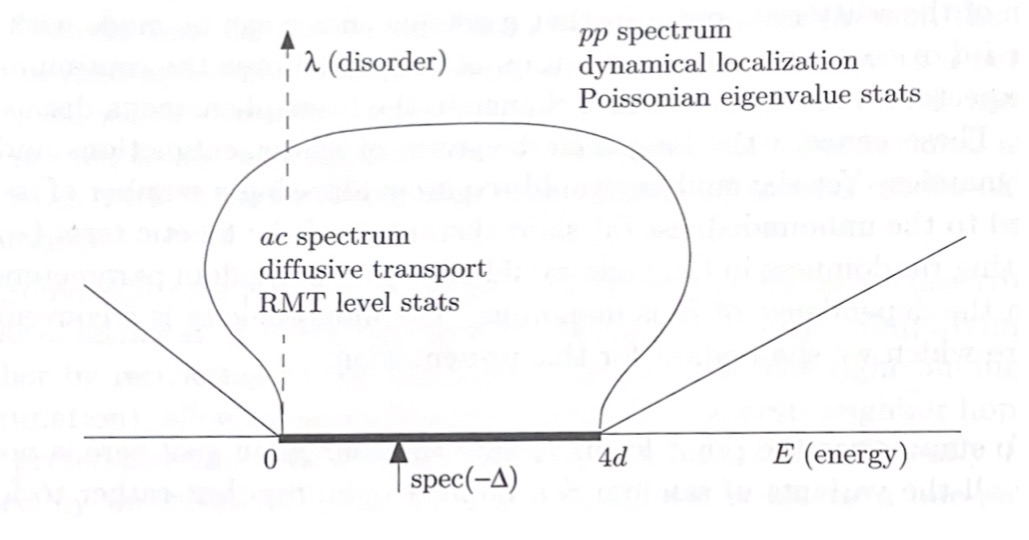
\includegraphics[width=0.6\textwidth]{IMG_1072.jpeg}
    \caption{Picture from \cite{aizenman2015}}
    \label{fig:nome_etichetta}
\end{figure}


\clearpage
\chapter{Localization properties}
We have understood what localization means from a heuristic point of view. In the previous chapter, it was presented as a spectral property of the Hamiltonian. In this section, we introduce dynamical properties for localization and discuss the implications between them. The definitions follow those given by A. Klein in \cite{klein2007}.

\section{Types of localization}

\begin{definition}[Spectral localization]
We say that $H_{\omega,\alpha}$ exhibits \textbf{spectral localization} if it has pure point spectrum almost surely. That is,
\begin{equation}
    \sigma(H_{\omega,\alpha}) = \sigma_{\mathrm{pp}}(H_{\omega,\alpha}) \quad \text{and} \quad \sigma_{\mathrm{c}}(H_{\omega,\alpha}) = \emptyset    
\end{equation}
for almost every realization of $\omega \in \Omega$.
\end{definition}


\begin{definition}[Dynamical localization]
    We say that $H_{\omega,\alpha}$ exhibits dynamical localization if for all $p>0$ and $\phi \in \ell^2(\mathbb{Z}^d)$ of finite support,
    \begin{equation}
    \sup_{t \in \mathbb{R}} \left\| |X|^p\,e^{-it H_{\omega,\alpha}}\phi \right\| < \infty \label{eq:dynloc}
    \end{equation}
    for almost every realization of $\omega \in \Omega$, where the position operator $|X|$ is defined by $(|X|\phi)(n) = |n|\phi(n)$.
\end{definition}
\begin{remark}
    Furthermore, we can prove the following Preposition.
\end{remark}
\begin{proposition}\label{prop:dynloccute}
    Let $H_{\omega, \alpha}$ be a bounded random Schr\"odinger operator. If \eqref{eq:dynloc} holds, then $$\sum_{x \in \mathbb{Z}^d} |x|^{2p} | e^{-itH_{\omega,\alpha}}(0,x)|^2 < \infty$$
\end{proposition}
\begin{proof}
    Assume that $\psi(k) = 0$ for $|k| > R$ (i.e., $\psi$ has finite support). Then
\begin{align*}
    \||X|^p e^{-itH_{\omega,\alpha}} \psi\|^2 &= \sum_x |\langle \delta_x, |X|^p e^{-itH_{\omega,\alpha}} \psi \rangle|^2\\
    &= \sum_x |x|^{2p} \left|\sum_{|k|\le R}  e^{-itH_{\omega,\alpha}}(k,x) \psi(k)\right|^2\\
\end{align*}
Assume that the particle is intially localized in the origin (\textit{recall: we work under translation invariance}). Then we obtain $$ = \sum_x |x|^{2p} \left|\sum_{|k|\le R}  e^{-itH_{\omega,\alpha}}(k,x) \delta_0 \right|^2 =\sum_x |x|^{2p} | e^{-itH_{\omega,\alpha}}(0,x)|^2$$
\end{proof}

\begin{definition}[Exponential localization]
    We say that $H_{\omega,\alpha}$ exhibits exponential localization if 
    \begin{equation}
        \mathbb{E}\left( \sup_{t \in \mathbb{R}} |\langle \delta_0, e^{-itH_\omega} \delta_x \rangle |\right) \leq C e^{- \mu |x|}\label{eq:explocalisation}
    \end{equation}
    for all $x \in \mathbb{Z}^d$.
\end{definition}

\begin{remark}
Dynamical localization implies that all spatial moments of the distance are bounded uniformly in time. (Recall that because we are working on an infinite grid with translation invariance, we can consider any arbitrary starting site just as easily as the origin $0$). 

From \eqref{eq:dynloc}, we can already deduce that the probability of transitioning from $0$ to $x$ goes to zero faster than any polynomial, but \eqref{eq:explocalisation} makes this explicit with a direct exponential bound. In fact, the two definitions are strongly related, and we can prove the following implication.
\end{remark}

\begin{proposition}\label{prop:exptodyn}
Exponential localization implies that all moments of the position operator are bounded in time for almost every realization of $V_\omega$, i.e., it implies dynamical localization. 
\end{proposition}

\begin{proof}
To see how \eqref{eq:dynloc} follows from \eqref{eq:explocalisation}, we start from the result of Proposition \ref{prop:dynloccute} and the fact that $|e^{-itH_{\omega,\alpha}}(0,x)| \le 1$. It follows
\begin{align}
    \mathbb{E}\left(\sup_{t \in \mathbb{R}} \||X|^p e^{-itH_{\omega,\alpha}} \psi\|^2\right) &\le \sum_x |x|^{2p}\,\, \mathbb{E}\left(\sup_{t \in \mathbb{R}} |e^{-itH_{\omega,\alpha}}(0,x)|^2\right)\\ \nonumber
    &\le \sum_x |x|^{2p}\,\, \mathbb{E}\left(\sup_{t \in \mathbb{R}} |e^{-itH_{\omega,\alpha}}(0,x)|\right)\\ \nonumber
    &\le C \sum_x |x|^{2p} e^{-\mu|x|} \\
    &< \infty.\nonumber
\end{align}
\end{proof}

\begin{remark}
    Dynamical localization holds \textit{almost surely} rather than for every single realization because our bounds control only the \textit{expected} value over the disorder.
\end{remark}
\begin{lemma}\label{lemma:almostsurely}
    Let $(X, \mathcal{A}, \mu)$ be a measure space and $f: X \to [-\infty, \infty]$ measurable. If $\int_X |f| \, d\mu < \infty$, then $|f| < \infty$ $\mu$-almost everywhere, i.e. $\mu(\{x \in X : |f(x)| = \infty\}) = 0$.
\end{lemma}

\begin{proof}
    We proceed by contradiction. Let $A = \{x \in X : |f(x)| = \infty\}$ and assume $\mu(A) > 0$. 
    Because $|f|$ is a non-negative function, the integral over the entire space $X$ must be greater than or equal to the integral over $A$. Therefore, 
    \begin{align*}
        \int_{X} |f(x)| \, d\mu(x) &\ge \int_{A} |f(x)| \, d\mu(x) \\
        &= \int_{A} \infty \, d\mu(x) \\
        &= \infty \cdot \mu(A).
    \end{align*}
    
    Since we assumed $\mu(A) > 0$, the product $\infty \cdot \mu(A)$ is exactly $\infty$, which directly contradicts our initial hypothesis that $\int_{X} |f(x)| \, d\mu(x) < \infty$. 
    Therefore $\mu(A) = 0$, which precisely means that $|f(x)| < \infty$ almost everywhere.
\end{proof}






\clearpage 
\chapter{Fractional moments}
In this section, we introduce the key lemmas and theorems that help us prove localization. The goal of this section is to demonstrate the power of the fractional moments method (FMM). First, we define the Green function, and then we prove the first fractional bound: the \textit{a priori bound}. This will provide a good example of how we use simple but important analytic tools, such as the \textit{resolvent identity}. Finally, we will prove that localization holds on some conditions on the disorder parameter, using the bound on the fractional power of the Green function. Most of the proof are taken from \cite{stolz2011} and \cite{disertori2024}.
\section{The Green function}

The \emph{resolvent operator} is defined as:
\begin{equation}
    G_{z,\alpha} \coloneqq (H_{\omega,\alpha} - z)^{-1}
\end{equation}
and is a well-defined bounded operator for all $z \in \mathbb{C} \setminus \mathbb{R}$.\\

The following three lemmas are the most important tools in the main proofs of this thesis.
\begin{lemma}[Resolvent identity]
    For a linear operator $A: \mathcal{D}(A) \rightarrow \mathcal{H}$ and $z_1,z_2 \in \varrho(A)$, 
    $$ (A-z_1)^{-1} - (A- z_2)^{-1} = (A-z_1)^{-1}(z_1 - z_2)(A-z_2)^{-1}. $$ 
    Moreover, if $B: \mathcal{D}(B)\rightarrow \mathcal{H}$ shares a common domain with $A$ such that $\mathcal{D}(A)=\mathcal{D}(B)$, then
    $$ (A-z)^{-1} - (B- z)^{-1} = (A-z)^{-1}(B-A)(B-z)^{-1} $$ 
    for any $z \in \varrho(A) \cap \varrho(B)$.
\end{lemma}

\textit{The resolvent identity follows directly from simple algebraic manipulation of the inverses.}


\begin{lemma} \label{lemma:1/imz}
    For a self-adjoint operator A,
    \begin{equation}
        \left\| (A-z)^{-1} \right\| \le \frac{1}{\mathrm{Im}(z)}
    \end{equation}
    for all $ z \in \mathbb{C} \setminus \mathbb{R}$.
\end{lemma}
\begin{proof}
    For the definition of the operator norm, we know that 
    \[
    \left\|(A-z)^{-1}\right\| \coloneq \sup_{ \mu \in \sigma((A-z)^{-1})} |\mu|
    \]
    Let's consider a $ \lambda \in \mathbb{C}$ and write $ \mu = \frac{1}{\lambda -z}$. This means:
    \begin{align*}
    \frac{1}{\lambda-z} \in \sigma((A-z)^{-1}) &\iff (A-z)^{-1} - (\lambda-z)^{-1} \text{ not invertible} \\
    &\iff (A-z)^{-1} (A-\lambda)(\lambda-z)^{-1} \text{ not invertible} \\
    &\iff (A- \lambda) \text{ not invertible} \\
    &\iff \lambda \in \sigma(A)
    \end{align*}
    Where the resolvent identity has been used in second implication.\\
    Finally we obtain: 
    \[
    \left\|(A-z)^{-1}\right\| = \sup_{ \lambda \in \sigma(A)} \frac{1}{|\lambda -z|} = \frac{1}{\inf_{\lambda \in \sigma(A)} |\lambda-z|} = \frac{1}{\text{dist}(\sigma(A),z)}
    \]
    For a bounded and self-adjoint operator, we know that the spectrum is real-valued. For $ z \in \mathbb{C} \setminus \mathbb{R} $ the minimum distance between $ z$ and $ \sigma(A)$ is the imaginary component of $z$:\\
    \begin{equation}
        \left\|(A-z)^{-1}\right\| \le \frac{1}{|\mathrm{Im}(z)|}
    \end{equation}
    
    
    
\end{proof}
The \textit{a priori bound} is a central estimate for the main proof in Section \ref{sec:SAW}. It provides a preliminary bound for the fractional moments of the Green function, and it holds for all values of $\alpha$.
\begin{lemma}[A priori bound] \label{lemma:aprioribound}
Let $s \in (0,1)$ and $\alpha \in (0,1]$. Then it holds
\begin{equation}
\mathbb{E}_{x}(|G_{z,\alpha}(x, x)|^s) \le \frac{1}{(1-s) \,\lambda^{s}}
\end{equation}
for all $x \in \mathbb{Z}^d$, $z \in \mathbb{C} \setminus \mathbb{R}$, and $\lambda > 0$.
\end{lemma}

\begin{proof}[Proof of the a priori bound]
For a fixed $x \in \mathbb{Z}^d$, we write $\omega = (\hat{\omega}, \omega_x)$, where $\hat{\omega}=(\omega_n)_{n \in \mathbb{Z}^d \setminus \{x\}}$ . We can separate the dependence of $H_{\omega,\alpha}$ on $\omega_x$ and $\hat{\omega}$ as follows :
\[
H_{\omega,\alpha} = (-\Delta)^\alpha + \lambda V_{\hat{\omega}} + \lambda \omega_x \chi_{\{x\}} = H_{\hat{\omega},\alpha} +  \lambda \omega_x \chi_{\{x\}}.
\]
For the operators $(H_{\omega,\alpha}-z)$ and $(H_{\hat{\omega},\alpha}-z)$, the resolvent identity yields 
\begin{equation}
(H_{\omega,\alpha} - z)^{-1} = (H_{\hat{\omega},\alpha} - z)^{-1} -  \lambda \omega_x ( H_{\hat{\omega},\alpha} - z)^{-1} \chi_{\{x\}} (H_{\omega,\alpha} - z)^{-1}.
\end{equation}
Taking the matrix elements, it follows
\begin{equation}
 G_{z,\alpha}(x, x) =  \hat{G}_{z,\alpha}(x, x) - \lambda \omega_x  \hat{G}_{z,\alpha}(x, x)  G_{z,\alpha}(x, x),
\end{equation}
where $ \hat{G}_{z,\alpha}$ denotes the Green function of $H_{\hat{\omega},\alpha}$ . Solving for $ G_{z,\alpha}(x, x)$, we obtain
\begin{equation}
 G_{z,\alpha}(x, x) = \frac{1}{a + \lambda \omega_x} \quad \text{with } a = \frac{1}{ \hat{G}_{z,\alpha}(x, x)}.
\end{equation}
Note that this expression is well-defined because $ \hat{G}_{z,\alpha}(x, x)$ cannot be zero. We can verify this quickly by applying the resolvent identity to the self-adjoint $H_{\hat{\omega},\alpha}$ for $z$ and $\bar{z}$ to extract its imaginary part:
\begin{align*}
    2i \, \mathrm{Im} \hat{G}_z(x,x) &= \langle e_x, \left[ (H_{\hat{\omega},\alpha}-z)^{-1} - (H_{\hat{\omega},\alpha}-\bar{z})^{-1} \right] e_x \rangle \\
    &= (z - \bar{z}) \langle (H_{\hat{\omega},\alpha}-\bar{z})^{-1} e_x, (H_{\hat{\omega},\alpha}-\bar{z})^{-1} e_x \rangle \\
    &= 2i \, \mathrm{Im}(z) \left\| (H_{\hat{\omega},\alpha}-\bar{z})^{-1} e_x \right\|^2.
\end{align*}
Since the squared norm is strictly positive, $\mathrm{Im} \hat{G}_z(x,x)$ always shares the same sign as $\mathrm{Im}(z)$. Therefore, whenever $\mathrm{Im}(z) > 0$, we strictly have $\mathrm{Im}  \hat{G}_{z,\alpha}(x, x) > 0$.\\

The crucial fact is that the complex number $a$ does not depend on $\omega_x$ . Thus, defining the partial expectation over the single site $x$ as $\mathbb{E}_x(\dots) := \int \dots \rho(\omega_x)\, d\omega_x$, and using the uniform density $\rho(\omega_x) = \frac{1}{2} \chi_{[-1,1]}$, we find 
\begin{equation}
\mathbb{E}_x(| G_{z,\alpha}(x, x)|^s) = \frac{1}{2 \lambda^s} \int_{-1}^{1} \frac{d\omega_x}{\left|\frac{a}{\lambda} + \omega_x\right|^s} \le \frac{1}{2 \lambda^s} \int_{-1}^{1} \frac{d\omega_x}{|\omega_x|^s} = \frac{1}{(1-s)\lambda^s}.
\end{equation}
The resulting constant $\frac{1}{1-s}$ is independent of $\lambda$ and $a$, and therefore independent of the remaining random variables $\hat{\omega}$, the energy $z$, and the site $x$ .
\end{proof}

\section{Localization at large disorder}

The primary goal of this thesis is to use self-avoiding walks, combined with FMM, in order to prove the following theorems.
\begin{theorem}[Schenker \cite{schenker2015}] \label{thm:theorem1.1}
Let $\alpha =1 $ and $s \in (0,1)$. Then for all $\lambda > \lambda_0(s)$,
\begin{equation}
\mathbb{E}\left(| G_{z, \alpha}(x,y)|^s\right) \le \frac{C}{(1-s)\lambda^s} e^{-\mu|x - y|}\qquad \forall\, x, y \in \mathbb{Z}^{d},\; x \ne y,\label{eq:schenkerbound}
\end{equation}
uniformly in $z \in \mathbb{C}\setminus \mathbb{R}$ with $C < \infty$ and $\mu >0$.
\end{theorem}

\begin{theorem}[Disertori, Escobar, Rojas-Molina \cite{disertori2024}]\label{thm:theorem1.2}
    Let $\alpha \in (0,1)$ and $s \in (\frac{d}{d+2\alpha},1)$. Then for all $\lambda > \lambda_0(s)$
    \begin{equation}
    \mathbb{E}[| G_{z,\alpha}(x,y)|^{s}] \le \frac{K}{(1-s)\lambda^{s}} \frac{1}{|x-y|^{s(d+2\alpha)}} \qquad \forall\, x, y \in \mathbb{Z}^{d},\; x \ne y, \label{eq:LRSAW}
    \end{equation}
uniformly in $z \in \mathbb{C} \setminus \mathbb{R}$ with $K < \infty$.
\end{theorem}
\begin{remark}
    In both theorems, we encounter the condition on the disorder parameter $\lambda > \lambda_0(s)$. For both scenarios, $\lambda_0(s) \coloneqq \left(\frac{1}{(1-s)\, R_{\chi^D}}\right)$. In particular, for $\alpha=1$, it has been proven by Schenker in \cite{schenker2015}, that $\lambda_0(s)$ is the unique solution of $\lambda_0= \mu_d \, e\,\ln(\lambda_0)$, where $R_{\chi^D}=1/\mu_d$ is a definition from the self-avoiding walks representations (see Section \ref{sec:SAW}).
\end{remark}


\subsection{From fractional moments to localization}


In this subsection we aim to prove localization, namely spectral localization for $\alpha \in (0,1]$ (Theorem \ref{thm:simonwolfftheorem}), and exponential localization for $\alpha =1$ (Theorem \ref{thm:explocproof}). In particular, we will also see that for $\alpha \in (0,1)$ a partial form of dynamical localization holds (Theorem \ref{thm:almostdynloc}).
 
\subsection*{Spectral localization}
We obtain spectral localization for all $\alpha \in (0,1]$ through the Simon-Wolff criterion.
\begin{proposition}[Simon-Wolff criterion]\label{proposition:simonwolff}
    Let $H_{\omega,\alpha}$ be a random operator in $l^2(\mathbb{Z}^d)$ with a random potential whose conditional-single site distribution is absolutely continuous. Then if for Lebesgue-almost every $E\in\mathbb{R}$ and $\mathbb{P}$-almost all $\omega$: 
    \begin{equation}
        \lim_{\eta \downarrow 0}\sum_{y \in \mathbb{Z}^d}|G_{E+i\eta,\alpha}(x,y)|^2 < \infty
    \end{equation}
    $H_{\omega,\alpha}$ has only pure point spectrum.
\end{proposition}
Proof can be found in \cite[Chapter 5]{aizenman2015}
\begin{theorem}\label{thm:simonwolfftheorem}
    Let Theorem \ref{thm:theorem1.1} and \ref{thm:theorem1.2} and  hold. Then, the spectrum of $H_{\omega,\alpha}$ consists only of pure point spectrum for a.e. realisation of $V_\omega$.
\end{theorem}
\begin{proof}[Proof from \cite{disertori2024}]
    From the Theorems \ref{thm:theorem1.1} and \ref{thm:theorem1.2} we notice that for all $\lambda>\lambda_0$:
    \begin{equation}
        \sum_{y \in \mathbb{Z}^d} \mathbb{E}[|G_{E+i\eta,\alpha}(x,y)|^s] = \frac{C}{(1-s)\lambda^s} \sum_{y \in \mathbb{Z}^d} e^{-\mu |x-y|} < \infty \quad \text{for all }\mu>0 \label{eq:4.20}
    \end{equation}
    and
    \begin{align}\label{eq:4.202}
        \sum_{y \in \mathbb{Z}^d} \mathbb{E}[|G_{E+i\eta,\alpha}(x,y)|^s] &= \frac{K}{(1-s)\lambda^{s}} \sum_{y \in \mathbb{Z}^d} \frac{1}{|x-y|^{s(d+2\alpha)}} \\ \nonumber
        &< \infty \quad \text{for all } s \in (\frac{d}{d+2\alpha},1) 
    \end{align} 
    uniformly for $z \in \mathbb{C} \setminus \mathbb{R}$ and $x \in \mathbb{Z}^d$ fixed.\\
    From Preposition \ref{proposition:squaredbound} we notice also that  $\sum_{y \in \mathbb{Z}^d} \mathbb{E}[|G_{E+i\eta,\alpha}(x,y)|^2]$ always exists but might be infinite for $\eta \rightarrow 0$.
    We argue:
    \begin{align*}
        \mathbb{E}\left[ \left( \lim_{\eta \downarrow 0} \sum_{y \in \mathbb{Z}^{d}} |G_{E+i\eta,\alpha}(x,y)|^{2} \right)^{\frac{s}{2}} \right] 
        &= \mathbb{E}\left[ \lim_{\eta \downarrow 0} \left( \sum_{y \in \mathbb{Z}^{d}} |G_{E+i\eta,\alpha}(x,y)|^{2} \right)^{\frac{s}{2}} \right] \\
        &\le \mathbb{E}\left[ \lim_{\eta \downarrow 0} \sum_{y \in \mathbb{Z}^{d}} |G_{E+i\eta,\alpha}(x,y)|^{s} \right] \\
        &\le \liminf_{\eta \downarrow 0} \sum_{y \in \mathbb{Z}^{d}} \mathbb{E}[|G_{E+i\eta,\alpha}(x,y)|^{s}] < \infty,
    \end{align*}
    where in the first two steps we used that the function $x \mapsto x^{\frac{s}{2}}$ is monotone and $\left|\sum_{n} a_{n}\right|^{s} \le \sum_{n} |a_{n}|^{s}$ for all $a_{n} \ge 0$ and $0 < s < 1$. The last two inequalities follow by Fatou and \eqref{eq:4.20} and \eqref{eq:4.202}. 
\end{proof}

\subsection*{Dynamical localization}
In order to prove the next theorems, we need the following definition.
\begin{definition}
    Let $\Sigma$ be the almost sure spectrum of $H_{\omega,\alpha}$. Then we call
    \begin{equation}
        Q(x,y,\Sigma) \coloneqq \sup_{\substack{g \in C_c(\Sigma) \\ |g| \le 1}} | g(H_{\omega,\alpha})(x,y)|
    \end{equation}
    the \textit{eigenfunction correlator}, for all $x,y \in \mathbb{Z}^d$.
\end{definition}
\begin{remark}
    Note that $$\sup_{t\in\mathbb{R}}|e^{-itH_{\omega,\alpha}}(0,x)|^2 \le \sup_{\substack{g \in C_c(\Sigma) \\ |g| \le 1}} | g(H_{\omega,\alpha})(o,x)| =: Q(x,0,\Sigma)$$
\end{remark}
The following Proposition, is the mein step for the proofs of Theorem \ref{thm:explocproof} and Theorem \ref{thm:almostdynloc}.
\begin{proposition}\label{prop:almostloc}
    Let $\Sigma$ be the almost sure spectrum of $H_{\omega,\alpha}$. Then,
    \begin{equation}
        \mathbb{E}[Q(x,y;\Sigma)] \le C_s \lim_{|\eta| \downarrow 0} \int_\Sigma \mathbb{E}[|G(x,y;E+i\eta)|^s] \, dE
    \end{equation}
    with a finite constant $C_s < \infty$
\end{proposition}

\begin{theorem}\label{thm:explocproof}
    Let $\Sigma$ be the almost sure spectrum of $H_{\omega,\alpha}$. Then for $\alpha=1$ we obtain exponential (and consequently dynamical) localization.
\end{theorem}
\begin{proof}
    We apply Theorem \ref{thm:theorem1.1} and Proposition \ref{prop:almostloc}
    \begin{equation}
        \mathbb{E}[Q(x,0,\Sigma)] \le C_s\,\frac{C}{(1-s)\,\lambda^s}\lim_{|\eta| \downarrow 0} \int_\Sigma \mathbb{E}[e^{-\mu|x-y|}] \, dE \le C_s\, |\Sigma|\,\,\frac{C}{(1-s)\,\lambda^s} e^{-\mu|x-y|} 
    \end{equation}
    as we wanted.
\end{proof}

\begin{theorem}\label{thm:almostdynloc}
    Let $\Sigma$ be the almost sure spectrum of $H_{\omega,\alpha}$. Then for $\alpha \in (0,1)$ and $0 < \beta < 2\alpha_s$, we have for a.e. $\omega \in \Omega$
            \begin{equation}
            \sup_{t \in \mathbb{R}} \sum_{x \ne 0} |x|^{\beta} |e^{-itH_{\alpha,\omega}}(0,x)|^2 < \infty.
            \end{equation}
            In particular, if $\alpha > \frac{1}{2}$, the first moment of the wave function initially localized at the origin and evolving under the action of $H_{\alpha,\omega}$ is finite.
\end{theorem}
\begin{proof}
    We apply Theorem \ref{thm:theorem1.2} and Proposition \ref{prop:almostloc}, and obtain
    \begin{align*}
        \mathbb{E}[Q(x,0,\Sigma)] \le \frac{C_s K}{(1-s)\,\lambda^s} \sum_{x \ne 0} |x|^\beta \frac{1}{|x|^{d+2\alpha_s}} < \infty,
    \end{align*}
    which converges for all $\beta < s(d+2\alpha)-d$. Since $0 \le Q(x,0,\Sigma) \le 1$, we can conclude that for almost every $\omega \in \Omega$:
    \begin{align*}
        \sup_{t \in \mathbb{R}} \sum_{x \ne 0} |x|^\beta |e^{-itH_{\alpha,\omega}}(0,x)|^2 \le \sum_{x \ne 0} |x|^\beta Q_\omega(x,0)^2 \le \sum_{x \ne 0} |x|^\beta Q_\omega(x,0) < \infty,
    \end{align*}
    which yields the required dynamical bounds .
\end{proof}

\begin{proof}[Proof of Proposition \ref{prop:almostloc}]
    As we mentioned in DEFINITION, for open sets $\Sigma \subset \mathbb{R}$ $$Q(x,y,\Sigma) \coloneqq \sup_{\substack{g \in C_c(\Sigma) \\ |g| \le 1}} | g(H_{\omega,\alpha})(x,y)|$$. For $g \in C_c(\Sigma)$ and $\xi \in \mathbb{R}$
    \begin{equation*}
    g(\xi) = \lim_{\eta \downarrow 0} \frac{\eta}{\pi} \int \frac{g(E)}{(\xi - E)^2 + \eta^2} \, dE.
    \end{equation*}
    which for $|g| \le 1$ means
    \begin{equation}
        Q(x,y, \Sigma) \le \lim_{\eta \downarrow 0} \frac{1}{\pi} \int_{\Sigma} |\mathrm{Im}(G_{E + i\eta,\alpha})(x,y) | dE
    \end{equation}
    Averaging and applying Fatou's and Fubini's theorems we have
    \begin{equation} \label{eq:7.29}
        \mathbb{F}[Q(x,y;I) ]\le \liminf_{\eta \downarrow 0} \frac{1}{\pi} \int_I \mathbb{E}[|\mathrm{Im}(G_{E + i\eta,\alpha})(x,y)|] \, dE.
    \end{equation}
    By the Cauchy-Schwarz inequality
    \begin{equation} \label{eq:7.30}
        |\mathrm{Im}(G_{E + i\eta,\alpha})(x,y)| \le \sqrt{|\mathrm{Im}(G_{E + i\eta,\alpha})(x,x)| |\mathrm{Im}(G_{E + i\eta,\alpha})(y,y)|}.
    \end{equation}
    where $\mathrm{Im}(G_{E + i\eta,\alpha})(x,y) >0$ when $\eta>0$.\\
    Splitting the integrand in \eqref{eq:7.29} into powers $(1-s)$ and $s$ and applying \eqref{eq:7.30} to just the $s$ power we get
    \begin{equation} \label{eq:7.31}
        \begin{split}
        &\left( \int_I \mathbb{E}[|\mathrm{Im}(G_{E + i\eta,\alpha})(x,y)|] \, dE \right)^2 \\
        &= \left( \int_I \mathbb{E}\left[ |\mathrm{Im}(G_{E + i\eta,\alpha})(x,y)|^{1-s} |\mathrm{Im}(G_{E + i\eta,\alpha})(x,y)|^s \right] \, dE \right)^2 \\
        &\le \left( \int_I \mathbb{E}\left[ \left( |\mathrm{Im}(G_{E + i\eta,\alpha})(x,x)|^{\frac{1-s}{2}} |\mathrm{Im}(G_{E + i\eta,\alpha})(y,y)| \right)^{\frac{1-s}{2}} |\mathrm{Im}(G_{E + i\eta,\alpha})(x,y)|^s \right] \, dE \right)^2 \\
        &\le \int_I \mathbb{E}[|\mathrm{Im}(G_{E + i\eta,\alpha})(x,x)|^{1-s} |\mathrm{Im}(G_{E + i\eta,\alpha})(x,y)|^s] \, dE \\
        &\quad \times \int_I \mathbb{E}[|\mathrm{Im}(G_{E + i\eta,\alpha})(y,y)|^{1-s} |\mathrm{Im}(G_{E + i\eta,\alpha})(x,y)|^s] \, dE,
        \end{split}
    \end{equation}
    where we again applied the Cauchy-Schwarz inequality.
    Since we are working with under translation invariance, we focus now on bounding one of the integrals, knowing that everything holds for the other too.

    Using the subadditivity property $\left|\sum_{n} a_{n}\right|^{s} \le \sum_{n} |a_{n}|^{s}$  we estimate
    \begin{equation} \label{eq:7.32}
        |\mathrm{Im}(G_{E + i\eta,\alpha})(x,y)|^s \le \frac{1}{2^s} \left( |G_{E+i\eta,\alpha}(x,y)|^s + |G_{E-i\eta,\alpha}(x,y)|^s \right)
    \end{equation}
    The ratio $G(x,y;z) / G(x,x;z)$ is independent of $V(x)$ for any $z \in \mathbb{C} \setminus \mathbb{R}$[cite: 3]. It therefore coincides with the ratio[cite: 3]
    \[
        \frac{G(x,y;z)}{G(x,x;z)} = \frac{G_\nu(x,y;z)}{G_\nu(x,x;z)}
    \]
    of the Green function of the operator $H_\nu := H + (\nu - V(x))1_{\{x\}}$, in which the potential at $x$ is changed to the value $\nu$[cite: 3]. As a consequence, in its dependence on $V(x)$ the integrand in the first factor on the right in \eqref{eq:7.31} (after the application of \eqref{eq:7.32}) is bounded by[cite: 3]
    \begin{equation} \label{eq:7.33}
        \begin{split}
        &\frac{|\mathrm{Im}\, \Gamma(z)|^{1-s}}{|V(x) - \Gamma(z)|^{2-2s}} \frac{|\nu - \Gamma(z)|^s}{|V(x) - \Gamma(z)|^s} |G_\nu(x,y;z)|^s \\
        &\le (|\nu|^s + |\Gamma(z)|^s) \frac{|\mathrm{Im}\, \Gamma(z)|^{1-s}}{|V(x) - \Gamma(z)|^{2-2s}} \frac{1}{|V(x) - \Gamma(z)|^s} |G_\nu(x,y;z)|^s
        \end{split}
    \end{equation}
    with $\Gamma(z)$ the inverse negative Green function at $z$ of the operator $H$ in which the potential $V(x)$ is set to zero[cite: 3]. Conditioning on all random variables aside from $V(x)$, the conditional expectation is estimated with the help of Lemma 7.8, which, e.g., for the first term yields[cite: 3]
    \begin{equation} \label{eq:7.34}
        \mathbb{E}[|G(x,y; E+i\eta)|^s | \{V(y)\}_{y \neq x}] \le C_s (|\nu|^s + 1) |G_\nu(x,y; E+i\eta)|^s.
    \end{equation}
    The resulting inequality may now be averaged over $\nu$[cite: 3]. For its probability distribution we pick $(|\nu|^s + 1)^{-1} \rho_x(\nu|V_{\neq x}) / \int (|\nu'|^s + 1)^{-1} \rho_x(\nu'|V_{\neq x}) \, d\nu'$ as the density[cite: 3]. Note that the normalization is bounded away from zero[cite: 3]. This yields the claim for the first factor[cite: 3].

    For an application of the above inequality to the factors involving $E - i\eta$ we also note that $|\langle \delta_x, \mathrm{Im}(H - z)^{-1} \delta_x \rangle| = |\langle \delta_x, \mathrm{Im}(H - \bar{z})^{-1} \delta_x \rangle|$ for any $z \in \mathbb{C} \setminus \mathbb{R}$[cite: 3].
    This concludes the proof of the assertion[cite: 3].
\end{proof}

The next proposition establishes a correlation between the fractional and second moments.

\begin{lemma} \label{proposition:squaredbound}
For every $s \in (0,1)$ there exists a constant $C_1 \coloneqq C_1(s,\rho) < \infty$ such that
\begin{equation}
|\mathrm{Im}(z)| \, \mathbb{E}_x\left(|G_{z}(x,y)|^2\right) \le C_1 \, \mathbb{E}_x\left(|G_{z}(x,y)|^s\right)
\end{equation}
for all $z \in \mathbb{C} \setminus \mathbb{R}$ and $x, y \in \mathbb{Z}^d$.
\end{lemma}

\begin{remark}
    From this bound, we can obtain decay for the second moments as well. However, it is not per se sufficient to prove localization, due to the dependence on the factor $\frac{1}{|\mathrm{Im}(z)|}$, which (as we can see in Proposition \ref{proposition:simonwolff}) diverges as $z \to \mathbb{R}$.  
\end{remark}

\begin{proof}
As in the proof of Lemma \ref{lemma:aprioribound}, we consider the perturbed Hamiltonian
\[
H^{(\nu)} = H_{\omega,\alpha} + \nu \chi_{\{x\}}.
\]
Its Green's function will be denoted by $G^{(\nu)}_z$. Applying the resolvent identity, we find
\[
(H_{\omega,\alpha} - z)^{-1} = (H^{(\nu)} - z)^{-1} + \nu (H_{\omega,\alpha} - z)^{-1} \chi_{\{x\}} (H^{(\nu)} - z)^{-1}.
\]
Taking the matrix elements, this yields
\begin{equation}
    \begin{split}
        G_{z,\alpha}(x,y) &= G^{(\nu)}_z(x,y)+ \nu G_{z,\alpha}(x,y)G^{(\nu)}_z(x,x).
    \end{split}
\end{equation}
Solving for $G^{(\nu)}_z(x,y)$, we obtain
\begin{equation}
    \begin{split}
        G^{(\nu)}_z(x,y) &= \frac{G_{z,\alpha}(x,y)}{1 + \nu G_{z,\alpha}(x,x)} \\
        &= \frac{1}{\nu + G_{z,\alpha}(x,x)^{-1}} \cdot \frac{G_{z,\alpha}(x,y)}{G_{z,\alpha}(x,x)}. \label{eq:4.12}  
    \end{split}
\end{equation}

For the special case $x = y$ and $\tilde{\nu} = -\mathrm{Re}(G_{z,\alpha}(x,x)^{-1})$, we get from \eqref{eq:4.12} and Lemma \ref{lemma:1/imz} that
\[
\left|\frac{1}{\mathrm{Im}(G_{z,\alpha}(x,x)^{-1})}\right| = |G^{(\tilde{\nu})}_{z}(x,x)| \le \frac{1}{|\mathrm{Im}(z)|},
\]
which implies $|\mathrm{Im}(G_{z,\alpha}(x,x)^{-1})| \ge |\mathrm{Im}(z)|$. Inserting this bound into \eqref{eq:4.12} gives:
\begin{equation}
|\mathrm{Im}(z)| \, |G^{(\nu)}_z(x,y)|^2 \le \frac{|\mathrm{Im}(G_{z,\alpha}(x,x)^{-1})|}{|\nu + G_{z,\alpha}(x,x)^{-1}|^2} \cdot \frac{|G_{z,\alpha}(x,y)|^2}{|G_{z,\alpha}(x,x)|^2}.\label{eq:4.13}
\end{equation}

On the other hand, we can bound the exact same expression by summing over all sites $y' \in \mathbb{Z}^d$:
\begin{align}
|\mathrm{Im}(z)| \, |G^{(\nu)}_z(x,y)|^2 &\le |\mathrm{Im}(z)| \sum_{y' \in \mathbb{Z}^d} |G^{(\nu)}_z(x,y')|^2 \nonumber \\
&= |\mathrm{Im}(z)| \left\| (H^{(\nu)} - z)^{-1} e_x \right\|^2 \nonumber \\
&= |\mathrm{Im}(z)| \langle \delta_x, (H^{(\nu)} - \bar{z})^{-1} (H^{(\nu)} - z)^{-1} \delta_x \rangle. \nonumber 
\end{align}
Because $H_{\omega,\alpha}$ is a bounded, self-adjoint operator, $H^{(\nu)}$ is also bounded and self-adjoint (since the perturbation $\nu \in \mathbb{R}$ is finite). Applying the resolvent identity to $H^{(\nu)}$ for $z$ and $\bar{z}$ yields $(H^{(\nu)} - \bar{z})^{-1} (H^{(\nu)} - z)^{-1} = \frac{1}{2i\mathrm{Im}(z)} \left[ (H^{(\nu)} - z)^{-1} - (H^{(\nu)} - \bar{z})^{-1} \right]$. Substituting this into the inner product, we obtain:
\begin{align}
    |\mathrm{Im}(z)| \, |G^{(\nu)}_z(x,y)|^2 &\le |\mathrm{Im}(z)| \left\langle \delta_x, \frac{1}{2i\mathrm{Im}(z)} \left[ (H^{(\nu)} - z)^{-1} - (H^{(\nu)} - \bar{z})^{-1} \right] \delta_x \right\rangle \nonumber \\
    &= \frac{|\mathrm{Im}(z)|}{\mathrm{Im}(z)} \, \mathrm{Im}(G^{(\nu)}_z(x,x)) \nonumber \\
    &= |\mathrm{Im}(G^{(\nu)}_z(x,x))| \nonumber \\
    &= \frac{|\mathrm{Im}(G_{z,\alpha}(x,x)^{-1})|}{|\nu + G_{z,\alpha}(x,x)^{-1}|^2}, \label{eq:4.14}
\end{align}
where the final step uses \eqref{eq:4.12} evaluated at $x = y$.

For any $t \ge 0$ and $s \in (0,1)$, we have $\min(1, t^2) \le t^s$. Because the left-hand side $|\mathrm{Im}(z)| \, |G^{(\nu)}_z(x,y)|^2$ is bounded simultaneously by \eqref{eq:4.13} and \eqref{eq:4.14}, we can interpolate between the two bounds to obtain the following
\begin{equation}
|\mathrm{Im}(z)| \, |G^{(\nu)}_z(x,y)|^2 \le \frac{|\mathrm{Im}(G_z(x,x)^{-1})|}{|\nu + G_z(x,x)^{-1}|^2} \cdot \frac{|G_z(x,y)|^s}{|G_z(x,x)|^s}. \label{eq:4.15}
\end{equation}

We will now use the following ``re-sampling trick,'' which effectively introduces an additional random variable (here $\alpha$) to average over. For any non-negative Borel function $f$ on $\mathbb{R}$:
\begin{align}
\iint f(\omega_x + \nu) \rho(\omega_x + \nu)\, d\nu\, \rho(\omega_x)\, d\omega_x &= \iint f(\omega_x + \nu) \rho(\omega_x + \nu) \rho(\omega_x)\, d\omega_x\, d\nu \nonumber \\
&= \iint f(\omega_x) \rho(\omega_x) \rho(\omega_x - \nu)\, d\omega_x\, d\nu \nonumber \\
&= \int f(\omega_x) \rho(\omega_x) \left( \int \rho(\omega_x - \nu)\, d\nu \right) d\omega_x \nonumber \\
&= \int f(\omega_x) \rho(\omega_x)\, d\omega_x,\label{eq:4.16}
\end{align}
where we applied Fubini's theorem in the first and third steps, the translation invariance of the Lebesgue measure in the second step, and the fact that $\int \rho(\omega_x -\nu)\, d\nu = 1$ in the final step.

Choosing $f(\omega_x) = |G_{z,\alpha}(x,y)|^2$, equations \eqref{eq:4.15} and \eqref{eq:4.16} yield:
\begin{align}
|\mathrm{Im}(z)| \, \mathbb{E}_x(|G_{z,\alpha}(x,y)|^2) &= |\mathrm{Im}(z)| \, \mathbb{E}_x\left( \int |G^{(\nu)}_z(x,y)|^2 \rho(\omega_x + \nu)\, d\nu \right) \nonumber \\
&\le \mathbb{E}_x\left( |\mathrm{Im}(G_{z,\alpha}(x,x)^{-1})| \frac{|G_{z,\alpha}(x,y)|^s}{|G_{z,\alpha}(x,x)|^s} \int \frac{\rho(\omega_x + \nu)}{|\nu + G_{z,\alpha}(x,x)^{-1}|^2}\, d\nu \right).\nonumber
\end{align}

We now apply Lemma \ref{lemma:notveryuseful} (below) with $w = G_{z,\alpha}(x,x)^{-1}$ to conclude that:
\[
|\mathrm{Im}(z)| \, \mathbb{E}_x(|G_{z,\alpha}(x,y)|^2) \le C_1 \, \mathbb{E}_x(|G_{z,\alpha}(x,y)|^s),
\]
where the constant $C_2 < \infty$ depends only on the support of $\rho$, but is entirely independent of $x$, $y$, and $z$.
\end{proof}

\begin{lemma}\label{lemma:notveryuseful}
Let $0<s<1$. There exists a constant $C_1 \coloneq C_1(s) < \infty$ such that
\[
|\mathrm{Im}\, w| \cdot |w|^s \int \frac{\rho(\omega_x + \alpha)}{|\alpha + w|^2}\, d\alpha \le C_2
\]
uniformly in $w \in \mathbb{C}$ and $\omega_x \sim \mathcal{U}[-1,1]$.
\end{lemma}
\begin{proof}
Using the inequality $|w|^s \le |\nu|^s + |\nu + w|^s$, we can bound the integral by splitting it into two parts:

\begin{enumerate}
    \item \textbf{Bounding the first term:}
    \begin{align*}
    |\mathrm{Im}(w)| \int \frac{|\nu|^s \rho(\omega_x + \nu)}{|\nu + w|^2}\, d\nu &\le |\mathrm{Im}(w)| \int \frac{\left\| |\nu|^s \rho(\omega_x + \nu) \right\|_\infty}{|\nu + w|^2}\, d\nu \\
    &\le |\mathrm{Im}(w)| \left\| |\nu|^s \rho(\omega_x + \nu) \right\|_\infty \int \frac{1}{(\nu + \mathrm{Re}(w))^2 + \mathrm{Im}(w)^2}\, d\nu.
    \end{align*}
    Recall that for any $a,b \in \mathbb{R}$, we have the standard integral:
    \[
    \int_{-\infty}^{\infty} \frac{1}{a^2 + b^2}\, da = \frac{1}{b} \left[ \arctan\left(\frac{a}{b}\right) \right]_{-\infty}^{\infty} = \frac{\pi}{|b|}.
    \]
    For our uniform distribution $\rho = \frac{1}{2}\chi_{[-1,1]}$, the function is non-zero only when $\omega_x + \nu \in [-1,1]$. Since $\omega_x \in [-1,1]$, this forces $|\nu| = |\nu + \omega_x - \omega_x| \le 1 + 1 = 2$. Thus, we can bound the supremum:
    \begin{align*}
    |\mathrm{Im}(w)| \int \frac{|\nu|^s \rho(\omega_x + \nu)}{|\nu + w|^2}\, d\nu &\le \pi \left\| |\nu|^s \rho(\omega_x + \nu) \right\|_\infty \\
    &\le \pi \left( 2^s \cdot \frac{1}{2} \right) = \pi 2^{s-1}.
    \end{align*}

    \item \textbf{Bounding the second term:}
    Let $I_2 := |\mathrm{Im}(w)| \int \frac{\rho(\omega_x + \nu)}{|\nu + w|^{2-s}}\, d\nu$. We evaluate this in two regimes:
    
    \begin{enumerate}
        \item \textit{For large $|\mathrm{Im}(w)|$:} \\
        Since $|\nu + w| \ge |\mathrm{Im}(w)|$ and $\int \rho(\omega_x + \nu) \, d\nu = 1$, we have:
        $$I_2 \le |\mathrm{Im}(w)| \cdot \frac{1}{|\mathrm{Im}(w)|^{2-s}} \int \rho(\omega_x + \nu) \, d\nu = \frac{1}{|\mathrm{Im}(w)|^{1-s}}.$$
        
        \item \textit{For small $|\mathrm{Im}(w)|$:} \\
        Using the uniform bound $\rho \le \frac{1}{2}$, we substitute $u = \nu + \mathrm{Re}(w)$ to obtain:
        \begin{align*}
        I_2 &\le \frac{|\mathrm{Im}(w)|}{2} \int \frac{d\nu}{|\nu + w|^{2-s}} \\
        &= \frac{|\mathrm{Im}(w)|}{2} \int \frac{1}{(u^2 + \mathrm{Im}(w)^2)^{\frac{2-s}{2}}}\, du.
        \end{align*}
        Next, we substitute $t = \frac{u}{|\mathrm{Im}(w)|}$, which implies $du = |\mathrm{Im}(w)|\, dt$:
        \begin{align*}
        I_2 &\le \frac{|\mathrm{Im}(w)|^2}{2} \int \frac{1}{\left( |\mathrm{Im}(w)|^2 t^2 + \mathrm{Im}(w)^2 \right)^{\frac{2-s}{2}}}\, dt \\
        &= \frac{1}{2}\, |\mathrm{Im}(w)|^s \int \frac{1}{(t^2 + 1)^{\frac{2-s}{2}}}\, dt.
        \end{align*}
        
        To establish the finiteness of this constant, we consider the integral:
        \[
        C_s := \int_{-\infty}^{\infty} \frac{1}{(t^2 + 1)^{\frac{2-s}{2}}} \, dt.
        \]
        Because $s \in (0,1)$, the exponent satisfies $2 - s > 1$. This ensures the asymptotic decay $(t^2 + 1)^{-\frac{2-s}{2}} \sim |t|^{-(2-s)}$ as $|t| \to \infty$, rendering the integral absolutely convergent. 
    \end{enumerate}
    
    Combining both regimes for $I_2$, we see that it is bounded by a function that decays for large $|\mathrm{Im}(w)|$ and vanishes for small $|\mathrm{Im}(w)|$:
    \[
    I_2 \le \min\left( \frac{1}{|\mathrm{Im}(w)|^{1-s}}, \, \frac{C_s}{2} |\mathrm{Im}(w)|^s \right) \le C_s',
    \] 
    where $C_s'$ is a finite global constant. Combining Parts 1 and 2 completes the proof.
\end{enumerate}
\end{proof}

Now we can procede with the proof of the theorem.The proof, recalls the one proposed in \cite{stolz2011}

\begin{proof}[Proof of Theorem \ref{thm:theorem3}]
    
For $H_{\omega,\alpha}$ bounded and self-adjoint, from the spectral theorem ( see Definition \ref{def:spectralmeasuredef}), it exists a complex Borel spectral measure $\mu_{\delta_x, \delta_y} = \mu_{x,y}$ such that:
\[
\mu_{x,y}(B) := \langle \delta_x, \chi_B(H_{\omega,\alpha}) \delta_y \rangle.
\]
with $B$ Borel in $\mathbb{R}$. The \textit{total variation measure} $|\mu_{x,y}|$ is a ragular bounded Borel measure, and satisfies
\begin{equation}
    |\mu_{x,y}|(B) = \sup \sum_{i=1}^{\infty} | \mu_{x,y}|(B_j) \label{eq:deftotvar}
\end{equation}
where $B = \bigcup {B_j}$, with $B_j$ disjoint. For $\mu_{x,y}$ complex, there exists $\alpha_j$ complex, such that $|\mu_{x,y}(B_j)|= \alpha_j\,\mu_{x,y}(B_j)$ and $| \alpha_j | = 1$. Let $g \coloneq \sum_{j=1}^{\infty} \alpha_j \chi_{B_j}$, which implies that $\vert{}g\vert{} \le 1$. Then it holds:
\begin{equation}
   \left| \int_B g(\xi)\,\, d\mu_{x,y}(\xi)\right| = \left| \sum_{j=1}^{\infty} \alpha_j \mu_{x,y}(B_j) \right|= \sum_{j=1}^{\infty} |\mu_{x,y}|(B_j).
\end{equation}
From \ref{eq:deftotvar} we obtain:
\begin{align}
\label{eq:40}
|\mu_{x,y}|(B) &= \sup_{\substack{g: \mathbb{R} \to \mathbb{C} \text{ Borel} \\ |g|\le 1}} \left| \int_B g(\xi)\,\, d\mu_{x,y}(\xi) \right| \nonumber \\
&= \sup_{|g| \le 1} |\langle \delta_x, g(H_{\omega,\alpha})\chi_B(H_{\omega,\alpha}) \delta_y \rangle|,
\end{align}
e.g. \cite[Chapter 6]{rudin1987}. This implies for $g= e^{-itH_\omega}$: 
$$\sup_{t \in \mathbb{R}} |\langle \delta_x, e^{-itH_\omega} \chi_B(H_{\omega,\alpha}) \delta_y \rangle| \le |\mu_{x,y}|(B).$$ 
Therefore, Theorem \ref{thm:theorem2} will follow from a corresponding exponential decay bound for $\mathbb{E}(|\mu_{x,y}|(B))$.\\

From Lusin's theorem, we can extend the bound also for $g \in C_c(B)$: $$|\mu_{x,y}|(B) =  \sup_{\substack{g \in C_c(B) \\ |g| \le 1}} |\langle \delta_x, g(H_{\omega,\alpha}) \delta_y \rangle|.$$ for $B$ bounded \textcolor{red}{open} interval, which is exactly our case since we consider $\xi \in \sigma(H_{\omega,\alpha})$ bounded in $\mathbb{R}$.
For $g \in C_c(B)$ it follows (using that $g$ is bounded and uniformly continuous) that, uniformly in $\xi \in \mathbb{R}$,

\begin{equation*}
g(\xi) = \lim_{\eta \downarrow 0} \frac{\eta}{\pi} \int \frac{g(E)}{(\xi - E)^2 + \eta^2} \, dE.
\end{equation*}

Now, always assuming that $g \in C_c(B)$, by the spectral theorem (see Def. \ref{def:spectralmeasuredef}), dominated convergence and Fubini
\begin{align*}
    \langle \delta_x, g(H_{\omega,\alpha}) \delta_y \rangle &= \int_{\mathbb{R}} g(\xi) \, d\mu_{x,y}(\xi) \\
    &= \lim_{\eta \downarrow 0}\int_{\mathbb{R}} \left(   \frac{\eta}{\pi} \int_B \frac{g(E)}{(\xi - E)^2 + \eta^2} \, dE \right) d\mu_{x,y}(\xi)\\
    &= \lim_{\eta \downarrow 0} \frac{\eta}{\pi} \int_B g(E) \left(  \int_{\mathbb{R}}  \frac{1}{(\xi - E)^2 + \eta^2} \,d\mu_{x,y}(\xi) \right)dE  \\
    &= \lim_{\eta \downarrow 0} \frac{\eta}{\pi} \int_B g(E) \langle \delta_x,((H_{\omega,\alpha} - E)^2 + \eta^2)^{-1} \delta_y \rangle\, dE\\
    &= \lim_{\eta \downarrow 0} \frac{\eta}{\pi} \int_B g(E) \langle \delta_x, (H_{\omega,\alpha} - E - i\eta)^{-1}(H_{\omega,\alpha} - E + i\eta)^{-1} \delta_y \rangle\, dE
\end{align*}
Now we can bound $\mathbb{E}(|\mu_{x,y}|)$, considering that $|g(E)| \le 1$:
\begin{align*}
\mathbb{E}(|\mu_{x,y}|(B)) &\le \mathbb{E}\left( \lim_{\eta \downarrow 0} \frac{\eta}{\pi} \int_B g(E) \langle \delta_x, (H_{\omega,\alpha} - E - i\eta)^{-1}(H_{\omega,\alpha} - E + i\eta)^{-1} \delta_y \rangle\, dE \right) \\
&\le \mathbb{E}\left( \lim_{\eta \to 0^+} \frac{\eta}{\pi} \int_B \sum_{z \in \mathbb{Z}^d} |\langle \delta_x, (H_{\omega,\alpha} - E - i\eta)^{-1} \delta_z \rangle| |\langle \delta_z, (H_{\omega,\alpha}- E + i\eta)^{-1} \delta_y \rangle| \, dE \right) \\
&\le \lim_{\eta \to 0^+} \frac{1}{\pi} \int_B \sum_{z \in \mathbb{Z}^d} \left( \mathbb{E}(\eta |\langle \delta_x, (H_{\omega,\alpha}- E - i\eta)^{-1} \delta_z \rangle|^2) \right)^{1/2} \\
&\quad \cdot \left( \mathbb{E}(\eta |\langle \delta_z, (H_{\omega,\alpha} - E + i\eta)^{-1} \delta_y \rangle|^2) \right)^{1/2} dE,
\end{align*}
where, in this order, Fatou, Fubini and Cauchy--Schwarz (on $\mathbb{E}$) have been used. \\
We can use Proposition \ref{proposition:squaredbound} and the hypothesis to obtain
\begin{align*}
\mathbb{E}(|\mu_{x,y}|(B)) &\le \frac{C_1}{\pi} \int_B \sum_{z \in \mathbb{Z}^d} \left(\mathbb{E}|G_\omega(x,z; E+i\eta)|^s\right)^{1/2} \left(\mathbb{E}|G_\omega(z,y; E-i\eta)|^s\right)^{1/2} dE \\
&\le \frac{C_1 |B| C}{\pi} \sum_{z \in \mathbb{Z}^d} e^{-\frac{\mu}{2}|x-z|} e^{-\frac{\mu}{2}|z-y|}.
\end{align*}

By the triangle inequality, $\frac{\mu}{2}|x-z| + \frac{\mu}{2}|z-y| \ge \frac{\mu}{4}|x-y| + \frac{\mu}{4}|x-z| + \frac{\mu}{4}|z-y|$. Therefore,
\[
\mathbb{E}(|\mu_{x,y}|(B)) \le \left( \frac{C_1 |B| C}{\pi} \sum_{z \in \mathbb{Z}^d} e^{-\frac{\mu}{4}|x-z|} e^{-\frac{\mu}{4}|z-y|} \right) e^{-\frac{\mu}{4}|x-y|} \le \widetilde{C} e^{-\widetilde{\mu}|x-y|},
\]
\end{proof}

\subsection{Exponential decay of the eigenfucntions}
From \textit{exponential and dynamical localization}, we can obtain that all the eigenfunction of the time-evolving Schr\"odinger operator decay also exponentially. 
\begin{enumerate}
    \item da simon wolff ottengo Theorem 7.4
    \item dalla dynamical ottengo che decade più veloce di ogni polinomio
    \item dalla exponential so che la sua time evolution  
\end{enumerate}

\clearpage
\chapter{SAW representation}\label{sec:SAW}
INIZIA CON UNA INTRODUZIONE DI CAPITOLOOOOOOOOOO

\section{SAW Definitions}
\begin{definition}[Self-Avoiding Walk]
A \textbf{self-avoiding walk} on the integer lattice $\mathbb{Z}^d$ of length $N \in \mathbb{N}_0$ is an ordered $(N+1)$-tuple of distinct lattice sites
\[
\gamma = (\gamma_0, \gamma_1, \dots, \gamma_N) \in (\mathbb{Z}^d)^{N+1}
\]
such that consecutive vertices are nearest neighbors, that is,
\[
|\gamma_i - \gamma_{i-1}| = 1 \quad \text{for all } i \in \{1, \dots, N\},
\]
and $\gamma_i \ne \gamma_j$ for all $i \ne j$.
\end{definition}

\begin{figure}[ht!]
    \centering
    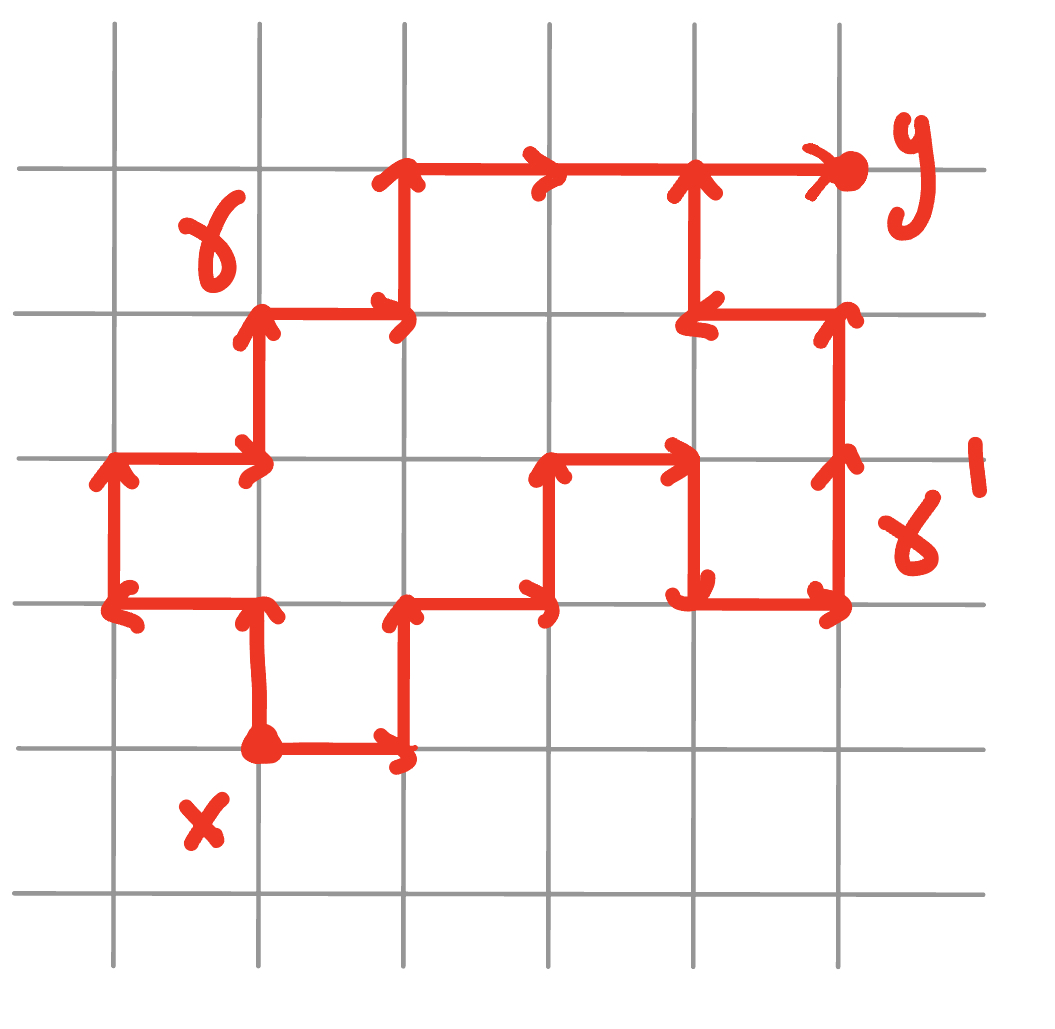
\includegraphics[width=0.5\textwidth]{IMG_0259.jpeg}
    \caption{$\gamma$ and $\gamma '$ are self-avoiding walks from $x$ to $y$}
\end{figure}


\begin{definition}[Sets of Self-Avoiding Walks]
Let $\Lambda \subseteq \mathbb{Z}^d$. For any $x, y \in \Lambda$ and $N \in \mathbb{N}_0$:
\begin{enumerate}
    \item[\textup{(i)}] $\mathcal{S}_N^{(\Lambda)}(y, x)$ denotes the set of all self-avoiding walks of length $N$ contained entirely in $\Lambda$, starting at $\gamma_0 = x$ and terminating at $\gamma_N = y$. When $\Lambda = \mathbb{Z}^d$, we simply write $\mathcal{S}_N(y, x)$.
    \item[\textup{(ii)}] $\mathcal{S}_N^{(\Lambda)}(x) := \bigcup_{y \in \Lambda} \mathcal{S}_N^{(\Lambda)}(y, x)$ denotes the set of all self-avoiding walks of length $N$ in $\Lambda$ starting at $x$.
    \item[\textup{(iii)}] $c_N := | \mathcal{S}_N(x)| = \sum_{y \in \mathbb{Z}^d} | \mathcal{S}_N(y, x)|$ denotes the total number of self-avoiding walks of length $N$ on $\mathbb{Z}^d$ originating from a fixed site (e.g., the origin $0$), which is independent of the starting vertex by translation invariance.
\end{enumerate}
\end{definition}

\begin{definition}[Connectivity Constant]
The \textbf{connective constant} (or connectivity constant) $\mu_d$ of the lattice $\mathbb{Z}^d$ is defined as the asymptotic growth rate of $c_N$:
\[
\mu_d := \lim_{N \to \infty} (c_N)^{1/N}.
\]
By subadditivity of $\log c_N$, this limit exists, is positive, and satisfies the strict inequality $\mu_d < 2d - 1$.
\end{definition}

\begin{claim}
Let $\mu_d$ be the connective constant (or growth rate) of self-avoiding walks on $\mathbb{Z}^d$. Then:
\[
\mu_d \le 2d - 1
\]
\end{claim}

\begin{proof}
Let $c_N$ denote the number of self-avoiding walks (SAWs) of length $N$ starting from the origin $0 \in \mathbb{Z}^d$, and let $S_N(0, x)$ denote the set of such walks ending at $x \in \mathbb{Z}^d$. By definition:
\[
c_N = \sum_{x \in \mathbb{Z}^d} |S_N(0, x)| = \sum_{x \in \mathbb{Z}^d} \sum_{\gamma \in S_N(0, x)} 1
\]
Consider the generating function (\textit{susceptibility}) with parameter $\beta >0$ in $\mathbb{C}$:
\[
\sum_{N=0}^{\infty} |\beta|^N c_N = \sum_{N=0}^{\infty} |\beta|^N \sum_{x \in \mathbb{Z}^d} |S_N(0, x)|
\]

For $N = 0$, $c_0 = 0$. For $N \ge 1$, a walk cannot immediately step back onto the previous vertex (non-reversing condition). Thus:
\begin{itemize}
    \item The first step has at most $2d$ choices.
    \item Each of the subsequent $N-1$ steps has at most $2d - 1$ choices.
\end{itemize}
This gives the upper bound:
\[
c_N \le 2d (2d - 1)^{N-1}, \quad \text{for } N \ge 1.
\]

Using this upper bound, we can bound the series from above:
\begin{align*}
\sum_{N=0}^{\infty} |\beta|^N c_N 
&\le \sum_{N=1}^{\infty} |\beta|^N (2d)(2d-1)^{N-1} \\
&= 2d |\beta| \sum_{k=0}^{\infty} |\beta|^k (2d-1)^k \quad (\text{setting } k = N-1) \\
&= 2d |\beta| \sum_{k=0}^{\infty} \left(|\beta|(2d-1)\right)^k
\end{align*}

This geometric series converges if and only if:
\[
|\beta|(2d - 1) < 1 \iff |\beta| < \frac{1}{2d - 1} =: R
\]
where $R = \frac{1}{2d - 1}$ is the radius of convergence of the bounding series.

By the Cauchy--Hadamard theorem, the radius of convergence $R'$ of the original series $\sum_{N=0}^{\infty} c_N |\beta|^N$ is:
\[
R' = \frac{1}{\limsup_{N \to \infty} c_N^{1/N}} = \frac{1}{\mu_d}
\]
Since the original series is bounded term-by-term by a series that converges for $|\beta| < R$, the true radius of convergence must satisfy:
\[
R' \ge R \implies \frac{1}{\mu_d} \ge \frac{1}{2d - 1}
\]
Taking the reciprocal yields:
\[
\mu_d \le 2d - 1.
\]
\end{proof}

\begin{definition}[SAW Correlation Function]
For a parameter $\\ \beta \ge 0$, the \textbf{self-avoiding walk correlation function} $C_\beta(y-x)$ between two vertices $x, y \in \mathbb{Z}^d$ is the generating function
\[
C_\beta(y - x) := \sum_{N=0}^\infty \beta^N \, |\mathcal{S}_N(y, x)|,
\]
defined for all values of $\beta$ for which the power series is absolutely convergent. By translation invariance, $C_\beta(y-x)$ depends only on the displacement vector $y - x$.
\end{definition}

\begin{definition}[SAW Susceptibility]
The \textbf{susceptibility} $\chi(\beta)$ of self-avoiding walks is the sum of the two-point correlation function over all endpoints:
\[
\chi(\beta) := \sum_{x \in \mathbb{Z}^d} C_\beta(x) = \sum_{N=0}^\infty c_N \, \beta^N.
\]
The series converges uniformly and absolutely if and only if $(c_N)^{1/N}\beta <1$, where the critical radius of convergence $R_\chi$ is given by $ \lim_{N \to \infty} \frac{1}{(c_N)^{1/N}}  = \frac{1}{\mu_d}$.
\end{definition}

\begin{proposition}[Exponential Decay of the Correlation Function]
Let $\beta \ge 0$ be such that $\beta < 1/\mu_d$. Then for every $\varepsilon > 0$ there exists a constant $K_\varepsilon < \infty$, independent of $x$, such that
\[
C_\beta(x) \;\le\; K_\varepsilon \big( (\mu_d+\varepsilon)\beta \big)^{|x|} \qquad \text{for all } x \in \mathbb{Z}^d.
\]
\end{proposition}

\begin{proof}
We know that $|\mathcal S_N(0,x)| = 0$ whenever $N < |x|$, and the sum defining $C_\beta(x)$ may be restricted to $N \ge |x|$:
\begin{equation}
    C_\beta(x) = \sum_{N=|x|}^{\infty} \beta^N \, |\mathcal S_N(x,0)| \;\le\; \sum_{N=|x|}^{\infty} \beta^N c_N.
\end{equation}

Fix $\varepsilon > 0$. Since $\mu_d = \lim_{N\to\infty} c_N^{1/N}$, by the definition of limit there exists $N_0  \in \mathbb{N}$ such that
\[
c_N^{1/N} < \mu_d + \varepsilon \qquad \text{for all } N \ge N_0,
\]
that is,
\[
c_N < (\mu_d+\varepsilon)^N \qquad \text{for all } N \ge N_0.   
\]
For $N = 0, 1, \dots, N_0-1$, define
\[
K_\varepsilon \;:=\; \max\left(1,\; \max_{0 \le N < N_0} \frac{c_N}{(\mu_d+\varepsilon)^N}\right),
\]
which is finite, being the maximum of finitely many finite quantities. By construction it holds:
\[
c_N \;\le\; K_\varepsilon (\mu_d+\varepsilon)^N \qquad \text{for all } N \ge 0.
\]

Combining it with (4.1) we obtain
\[
C_\beta(x) \;\le\; K_\varepsilon \sum_{N=|x|}^{\infty} \big[(\mu_d+\varepsilon)\beta\big]^N.
\]
Choosing $\varepsilon$ small enough that $r := (\mu_d+\varepsilon)\beta < 1$ (possible since $\beta < 1/\mu_d$), the tail of the geometric series equals
\[
\sum_{N=|x|}^{\infty} r^N = \frac{r^{|x|}}{1-r}.
\]
Hence
\[
C_\beta(x) \;\le\; \frac{K_\varepsilon}{1-(\mu_d+\varepsilon)\beta} \, \big[(\mu_d+\varepsilon)\beta\big]^{|x|}.
\]
where $ \dfrac{K_\varepsilon}{1-(\mu_d+\varepsilon)\beta}$ is still finite and indipendent from $x$.
\end{proof}


\section{SAW representation of $G_z$ }
The proof of the theorem 3.1 is similar to the one given by Schenker in []. We are going to work with the Green function defined on a volume
where one site is removed every stage. Therefore , for any $ \Lambda \subseteq \mathbb{Z}^d$ (finite or infinite) the Green function changes:
\begin{equation}
    G^{\Lambda}_z(x,y) \coloneq \begin{cases}
        (H^{\Lambda}_\omega -z), \qquad \forall x,y \in \Lambda\\
        0 \qquad,\, \text{otherwise}
    \end{cases}
\end{equation}
where $H^{\Lambda}_\omega -z \in \mathbb{C}^{\Lambda \times \Lambda}$ is the matrix obtained by restricting $ H_\omega -z$ to $ \Lambda$. In this thesis we will consider $ \Lambda = \mathbb{Z}^d$, but we leave the noation $\Lambda$ to highligth the fact that the same result holds for any volume.\\
To notice is also that  $H^{\Lambda}_\omega -z$ is still invertible for all $z \in \mathbb{C} \setminus \mathbb{R}$. In this section, for semplicity during calculations, we will write $ G^{\Lambda}(x,y)$ instead of $ G^{\Lambda}_z(x,y)$.

\begin{theorem}
Let $x, y \in \mathbb{Z}^d$, $x \neq y$, $\Lambda \subseteq \mathbb{Z}^d$. $G^\Lambda$ is defined as in (4.1). It holds
\begin{equation}
    G^\Lambda(x, y) =  \sum_{n=1}^N \sum_{\gamma \in \mathcal{S}_n(x, y)} \prod_{i=1}^n G^{\Lambda}(x, x) \cdot G^{\Lambda_i}(\gamma_i, \gamma_i) + R_N  \label{eq:SAWrep} 
\end{equation}

where $\Lambda_i = \Lambda \setminus \{x, \gamma_1, \dots, \gamma_{i-1}\}$ and
\begin{equation}
    R_N = \sum_{x \sim y} \sum_{\gamma \in \mathcal{S}_N(0, x)} \prod_{i=1}^{N-1} G^{\Lambda}(x, x) \cdot G^{\Lambda_i}(\gamma_i, \gamma_i) \cdot G^{\Lambda_N}(\gamma_N, y).    
\end{equation}

\end{theorem}
In order to prove Theorem 4.8, 
\vspace{.2cm}

\begin{claim} \label{claim:SAWrep}
\begin{equation}
    G^\Lambda(x, y) = G^\Lambda(x, x) \sum_{x_1 \sim x} G^{\Lambda_1}(x_1, y)
\end{equation}
\end{claim}
\begin{proof}
Using the resolvent identity for $A = (H_\omega^\Lambda - z)$ and $B = (H_\omega^{\{x\}} \oplus H_\omega^{\Lambda \setminus \{x\}} - z)$, we obtain:
\begin{align*}
&(H_\omega^\Lambda - z)^{-1} - (H_\omega^{\{x\}} \oplus H_\omega^{\Lambda \setminus \{x\}} - z)^{-1} \\
&= - (H_\omega^\Lambda - z)^{-1} \left( H_\omega^\Lambda - (H_\omega^{\{x\}} \oplus H_\omega^{\Lambda \setminus \{x\}}) \right) 
(H_\omega^{\{x\}} \oplus H_\omega^{\Lambda \setminus \{x\}} - z)^{-1}
\end{align*}

Moreover:
\[
H_\omega^\Lambda - (H_\omega^{\{x\}} \oplus H_\omega^{\Lambda \setminus \{x\}}) = -\sum_{x_1 \sim x}\delta_{x_1} =: T_{x, x_1}
\]

\noindent Now considering the matrix elements in $(x, y)$ with $x \neq y$ and matrix multiplication:
\[
\langle \delta_x, (H_\omega^\Lambda - z)^{-1} \delta_y \rangle - 0 = -\sum_{x_1, x_2} \langle \delta_x, (H_\omega^\Lambda - z)^{-1} \delta_{x_1} \rangle T_{x_1, x_2} \langle \delta_{x_2}, (H_\omega^{\{x\}} \oplus H_\omega^{\Lambda \setminus \{x\}} - z)^{-1} \delta_y \rangle
\]
For $T_{x_1, x_2} \neq 0$, we need $x_1 = x$ and $x_2 \sim x_1$.

Which leaves us with:
\[
G^\Lambda(x, y) = \sum_{x_1 \sim x} G^\Lambda(x, x)G^{\Lambda \setminus \{x\}}(x_1, y)
\]
\end{proof}
\begin{proof}[Proof of Theorem 5.8]
Now we separate the case in which $ x_1 =y$ (which implies $|x-y|=1$).
\[
G^\Lambda(x, y) = G^\Lambda(x, x) \left(\sum_{x_1 \sim x, x_1 \neq y}G^{\Lambda_1}(x_1, y) +  \delta_{|x-y|=1}\,G^{\Lambda_1}(y,y)\right)
\]
Iterating N times, it gives \eqref{eq:SAWrep}.
\end{proof}

\section{Proof with SAW}\label{subsec:Proofwithsaw}
In this las Section, we can use the SAW representation of the Green function \eqref{eq:SAWrep}, in order to prove Theorem \ref{thm:theorem1}.
\begin{proof}
We take the average of (4.2), and using  $|\sum a|^s \le \sum |a|^s$ (which follows from triangle inequality), we have:
\begin{align}
    \mathbb{E}\left[ |G^\Lambda(x, y)|^s \right] \le \sum_{n=1}^N \sum_{\gamma \in \mathcal{S}_n(x, y)} \mathbb{E}\left[ |G^\Lambda(x, x)|^s \prod_{i=1}^n |G^{\Lambda_i}(\gamma_i, \gamma_i)|^s \right] + \\
    \sum_{x \sim y} \sum_{\gamma \in \mathcal{S}_N(0, x)} \mathbb{E}[|G^{\Lambda}(x, x)|^s \prod_{i=1}^{N-1} |G^{\Lambda_i}(\gamma_i, \gamma_i)|^s \cdot |G^{\Lambda_N}(\gamma_N, y)|^s.]
\end{align}

The resolvent $G^{\Lambda_j}(w, w')$ does not depend on the random variables $\omega_{x_i}$, $i = 0, \dots, j-1$. Hence, recursive applications of the a priori bound (3.2) yield

\begin{align*}
\mathbb{E}\left[ |G^\Lambda(x, x)|^s \prod_{j=1}^n |G^{\Lambda_j}(\gamma_j, \gamma_j)|^s \right] 
\le \left( \frac{1}{1-s} \frac{1}{\lambda^s} \right)^{n+1}
\end{align*}

and
\begin{align*}
\mathbb{E}\left[ |G^\Lambda(x, x)|^s \prod_{j=1}^{N-1} |G^{\Lambda_j}(\gamma_j, \gamma_j)|^s \cdot |G^{\Lambda_{N-1}}(\gamma_N, y)|^s \right] \\
\le \left( \frac{1}{1-s} \cdot \frac{1}{\lambda^s} \right)^N \cdot \mathbb{E}\left[ |G^{\Lambda_{N-1}}(\gamma_N, y)|^s \right] 
\le  \left( \frac{1}{1-s} \frac{1}{\lambda^s} \right)^N  \frac{1}{|\mathrm{Im}(z)|^s}
\end{align*}

\noindent Where we used a priori bound and lemma 3.5.

\vspace{1em}
\noindent Inserting these estimates in the sums above, we get:
\begin{equation}
\mathbb{E}\left( |G^{(\Lambda)}(x,y)|^s \right) \le \sum_{n=0}^N \beta(s)^{1+n} |\mathcal{S}_n^{(\Lambda)}(y,x)| +  \text{\textit{Err}}(N) \frac{1}{|\mathrm{Im}(z)|^s} \label{eq:semifinalboundSAW}
\end{equation}
with $\text{\textit{Err}}(N) \coloneq \beta(s)^N |\mathcal{S}_N^{(\Lambda)}(x)|$ $ \beta(s) = {\frac{1}{1-s} \frac{1}{\lambda^s}}$
Let's consider the susceptability $\chi(\beta)$ of the self avoiding walks in $\mathcal{S}_N^{(\Lambda)}(x)$:
\begin{equation}
    \chi(\beta) = \sum_{x \in \mathbb{Z}^d} \sum_{N=0}^{\infty} \beta(s)^N \, |S_N^{(\Lambda)}(x)| = \sum_{N=0}^\infty c_N \, \beta(s)^N.
\end{equation}
The series converges absolutely if and only if $0 \le |\beta| < 1/\mu_d$, where $1/\mu_d = \lim_{N \rightarrow \infty} c_N ^{1/N}$ is the critical radius of convergence.
Thus, for $|\beta(s)| = \frac{1}{|(1-s)\lambda^s|}\le \frac{1}{\mu_d} $, $ \chi(\beta)$ converges uniformly, and most importantly:
\[
\text{\textit{Err}}(N) \longrightarrow 0 , \quad \text{for} \quad N \rightarrow \infty
\]
We send $N$ to the infinity and obtain from (4.7):
\begin{equation}
    \mathbb{E}\left( |G^{(\Lambda)}(x,y)|^s \right) \le \sum_{n=0}^\infty \beta(s)^{1+n} |\mathcal{S}_n^{(\Lambda)}(y,x)| 
\end{equation}

Taking the supremum over volumes $\Lambda$ now yields
\begin{equation}
\sup_{\Lambda \subset \mathbb{Z}^d} \mathbb{E}\left( |G^{(\Lambda)}(x,y)|^s \right) \le \beta(s) C_{\beta(s)}(x-y). \tag{4.3}
\end{equation}

It remains to establish for which $\lambda$ we may find $s \in (0,1)$ with $\beta(s) < 1/\mu_d$. As above, for $\lambda > e$ the unique critical point is $s_{\mathrm{crit}} = 1 - 1/\ln \lambda$ and
\[
\min_{s \in (0,1)} \beta(s) = \beta(s_{\mathrm{crit}}) = \frac{e \ln \lambda}{\lambda}
\] 
which is less than $1/\mu_d$ if and only if $\lambda > \lambda_{\mathrm{And}}$.
Finally we get:
\begin{equation}
\mathbb{E}\left(|G^{(\Lambda)}(x,y;z)|^{1 - \frac{1}{\ln \lambda}}\right) \le \beta(\lambda) K_\epsilon \ln \lambda \, e^{-m_\epsilon(\lambda)|x - y|}
\end{equation}
where
\[
m_\epsilon(\lambda) = -\ln \beta(\lambda) - \ln(\mu_d + \epsilon) > 0.
\]
\end{proof}

\clearpage
\chapter{Connection to Long-Range SAW}

The purpose of this chapter is to extend the self-avoiding walk representation of the resolvent, to random Hamiltonians with long-range hopping. In particular, we compare this setting with the previous model and apply the fractional moment method to study localization.\\
The difference lies in the kinetic operator, which is replaced by the fractional  discrete Laplacian $(-\Delta)^\alpha$ with $0<\alpha < 1$. This change leads to a polynomial decay bound for the avareged Green function, in sharp contrast with the standard exponential decay.\\
This chapter is based on the work of M. Disertori, R.M. Escobar and C. Rojas-Molina in 2024 \cite{disertori2024}.\\

\section{The fractional Laplacian}

\section{The SAW Representation for Long-Range Resolvents}
We consider the fractional Hamiltonian
\begin{equation}
H_{\alpha,\omega} = (-\Delta)^\alpha + \lambda V_\omega \quad \text{on } \ell^2(\mathbb{Z}^d),
\end{equation}
where $0 < \alpha < 1$ and $V_\omega$ is a diagonal matrix with i.i.d. random entries defined as in Section \ref{sec:The_Hamiltonian}.
The Green function $G_z = (H_{\alpha,\omega} - z)^{-1}$ is well-defined for all $z \in \mathbb{C} \setminus \mathbb{R}$, and its decay at strong disorder is closely related to the polynomial decay of the fractional Laplacian.\\

As before, in the long-range scenario, we use the geometric resolvent expansion to represent the fractional moments as a sum over self-avoiding paths and we obtain that the averaged fractional Green function satisfies
\begin{equation}
\mathbb{E}[|G_{z}(x,y)|^{s}] \le \frac{K_{0}}{(1-s)\lambda^{s}} \frac{1}{|x-y|^{d+2\alpha_{s}}} \qquad \forall\, x, y \in \mathbb{Z}^{d},\; x \ne y, \label{eq:LRSAW}
\end{equation}
uniformly in $z \in \mathbb{C} \setminus \mathbb{R}$, for all $\lambda > \lambda_0(s) \coloneq \left(\frac{1}{(1-s)R_{\chi^D}}\right)^{\frac{1}{s}}$. Here, $2\alpha_s \coloneq s(d+2\alpha)-d$ and $ \frac{1}{(1-s)\lambda^s}$ comes from the \textit{a priori bound}. \\

Since we are considring arbitrary sites on the lattice, we define the step weight kernel for the SAW as $D(x,y) \coloneq |(-\Delta)^\alpha(x,y)|^s$, which generates a transition probability $p(x \to y) \coloneq \frac{D(x,y)}{\sum_{z \ne x} D(x,z)}$ and is translation-invariant. 
This is well-defined for $s \in \left(\frac{d}{d+2\alpha}, 1\right)$ because the kernel is summable: $\sum_{x \ne 0} |(-\Delta)^\alpha(0,x)|^s < \infty$ ( See \eqref{eq:Dsbound}).
From this essential condition, we develop the same strategy as for the standard Anderson resolvent. The new definitions for SAWs are all generated by $D$.
\paragraph{SAW definitions for the  discrete Anderson model.}
Recall the definitions in Chapter 4. A self-avoiding walk (SAW) on the lattice $\mathbb{Z}^{d}$ with long-range jumps is characterized by the following essential components:

\begin{itemize}
    \item $\mathcal{S}_N(x,y)$ denotes the set of all self-avoiding walks of length $N$ starting at $\gamma_0 = x$ and terminating at $\gamma_N = y$. Due to the transaltion invariance of the fractional laplacian we know $\mathcal{S}_N(x,y) = \mathcal{S}_N(0,y-x)$ for all $x,y \in \mathbb{Z}^d$.
    \item \textbf{Two-point Function:} 
    $$C_{\beta}^{D}(x,y) = C_{\beta}^{D}(y-x) \coloneqq \sum_{n \ge 0} \beta^n \sum_{\gamma \in S_n(x,y)} \prod_{j=0}^{n-1} D(\gamma_j, \gamma_{j+1}),$$
    for all $x,y \in \mathbb{Z}^d$.
    \item \textbf{Susceptibility:} $$\chi^{D}(\beta)\coloneqq\sum_{x\in\mathbb{Z}^{d}}C_{\gamma}^{D}(x),$$ which is finite for values strictly below its radius of convergence $R_{\chi^{D}}$.
\end{itemize}
In particular, we also consideri the following consequences:
\begin{lemma}
    Consider the definitions given above. Then it holds $$ R_\chi^D \ge \frac{1}{\sum_{w\ne 0}D(0,w)} >0.$$
\end{lemma}
\begin{proof}
    For $n=2$, we have
$$
\sum_{x\in\mathbb{Z}^{d}}\sum_{\gamma\in\mathcal{S}_{2}(0,x)}D(0,\gamma_{1})D(\gamma_{1},x) = \sum_{\gamma_{1}\ne0}D(0,\gamma_{1})\sum_{x\ne 0, \gamma_{1}}D(\gamma_{1},x) 
$$
$$
\le \sum_{\gamma_{1}\ne0}D(0,\gamma_{1})\sum_{x\ne\gamma_{1}}D(\gamma_{1},x) = \left(\sum_{w\ne0}D(0,w)\right)^{2}.
$$
Repeating this argument inductively for any general length $n\ge1$, we obtain
$$
\sum_{x\in\mathbb{Z}^{d}}\sum_{\gamma\in\mathcal{S}_{n}(0,x)}\prod_{j=0}^{n-1}D(\gamma_{j},\gamma_{j+1})\le\left(\sum_{z\ne0}D(0,z)\right)^{n}.
$$
By substituting this bound into the definition of the susceptibility, we get a geometric series that converges as long as $\beta \sum_{z\ne0}D(0,z) < 1$. This guarantees that the radius of convergence satisfies
$$
R_{\chi^{D}}\ge\frac{1}{\sum_{z\ne0}D(0,z)}>0. \eqno{(3.7)}
$$
\end{proof}
\begin{proposition}
    Let $s \in (\frac{d}{d+2\alpha},1)$. Then 
    $$C_{\beta}^{D}(x,y) \le K_0 \frac{1}{|y-x|^{d+2\alpha_s}} $$ for all $x,y \in \mathbb{Z}^d$.\label{eq:twopointbound}
\end{proposition}
\textit{Proof in \cite[Lemma 4]{disertori2024}}.\\


As in the previous Chapter, we prove \eqref{eq:LRSAW} using a SAW representation of $G_{\alpha,\omega}$.
\begin{theorem}
    Let $s \in (\frac{d}{d+2\alpha},1)$. Then, for all the above definitions, it holds 
    \begin{equation}
        \mathbb{E}(|G_{\alpha,\omega}(x,y)|^s)\le\frac{1}{\lambda^{s}(1-s)}C_{\beta}^{D}(y-x)+\frac{1}{|\mathrm{Im}(z)|^{s}}\,R_{N}
    \end{equation}  
    for all $x,y \in \mathbb{Z}^d$. Moreover, 
    \begin{equation}
        R_N \coloneqq \left(\frac{1}{(1-s)\lambda^{s}}\right)^{N}\sum_{\gamma\in S_{N+1}(x,y)}\prod_{j=0}^{N-1}\,D(\gamma_{j},\gamma_{j+1}).
    \end{equation} 
\end{theorem}

\begin{proof}
    As in Chapter 4, we must work with Green functions defined on $\Lambda\subset\mathbb{Z}^{d}$, and to simplify the notation, we also set $\Delta^{\alpha}(x,y):=-(-\Delta)^{\alpha}(x,y)$, which guarantees $\Delta^{\alpha}(x,y)>0$ for all $x\ne y$ and $G_{\alpha,z}^{\Lambda}(x,y) = G^{\Lambda}(x,y)$. Recall also $\Lambda\backslash\{\gamma_{0},\dots,\gamma_{j-1}\} = \Lambda_j$. 

By the resolvent identity, we have for all $x\ne y \in\Lambda$
\begin{align*}
G^{\Lambda}(x,y) &= G^{\Lambda}(x,x)\Delta^{\alpha}(x,y)G^{\Lambda\backslash\{x\}}(y,y) \\
&\quad +G^{\Lambda}(x,x)\sum_{\gamma_{1}\in\Lambda\backslash\{x,y\}}\Delta^{\alpha}(x,\gamma_{1})G^{\Lambda\backslash\{x\}}(\gamma_{1},y).
\end{align*}
Repeating this expansion $N$ times and organizing the terms using the sets of self-avoiding walks $\mathcal{S}_{n}(x,y)$, we obtain
\begin{align*}
G^{\Lambda}(x,y) &= G^{\Lambda}(x,x)\left[\sum_{n=1}^{N}\sum_{\gamma\in\mathcal{S}_{n}(x,y)}\prod_{j=0}^{n-1}\Delta^{\alpha}(\gamma_{j},\gamma_{j+1})\prod_{j=1}^{n}G^{\Lambda_1}(\gamma_{j},\gamma_{j}) \right. \\
&\quad \left. +\sum_{\gamma\in\mathcal{S}_{N+1}(x,y)}\prod_{j=0}^{N-1}\Delta^{\alpha}(\gamma_{j},\gamma_{j+1})\prod_{j=1}^{N-1}G^{\Lambda_j}(\gamma_{j},\gamma_{j})G^{\Lambda_N}(\gamma_{N},y)\right].
\end{align*}Taking the fractional expectation $\mathbb{E}[|\cdot|^{s}]$ and utilizing the concavity of the function $v\mapsto v^{s}$ for $0<s<1$, we can pass the fractional power inside the sums
\begin{align*}
\mathbb{E}[|G^{\Lambda}(x,y)|^{s}] &\le \sum_{n=1}^{N}\sum_{\gamma\in\mathcal{S}_{n}(x,y)}\prod_{j=0}^{n-1}\Delta^{\alpha}(\gamma_{j},\gamma_{j+1})^{s}\cdot\mathbb{E}\left[|G^{\Lambda}(x,x)|^{s}\prod_{j=1}^{n}|G^{\Lambda_j}(\gamma_{j},\gamma_{j})|^{s}\right] \\
&\quad +\sum_{\gamma\in\mathcal{S}_{N+1}(x,y)}\prod_{j=0}^{N-1}\Delta^{\alpha}(\gamma_{j},\gamma_{j+1})^{s} \\
&\quad \cdot\mathbb{E}\left[|G^{\Lambda}(x,x)|^{s}\prod_{j=1}^{N-1}|G^{\Lambda_j}(\gamma_{j},\gamma_{j})|^{s}|G^{\Lambda_{N+1}}(\gamma_{N},y)|^{s}\right].
\end{align*}
The resolvent $G^{\Lambda_j}$ does not depend on the random variables $\omega_{\gamma_{i}}$ for $i=0,\dots,j-1$. Hence, we can apply the apriori bound recursively, which yields
\begin{align*}
\mathbb{E}\left[|G^{\Lambda}(x,x)|^{s}\prod_{j=1}^{n}|G^{\Lambda_j}(\gamma_{j},\gamma_{j})|^{s}\right] &\le \left(\frac{1}{(1-s)\lambda^{s}}\right)^{n+1}, \\
\mathbb{E}\left[|G^{\Lambda}(x,x)|^{s}\prod_{j=1}^{N-1}|G^{\Lambda_j}(\gamma_{j},\gamma_{j})|^{s}|G^{\Lambda_{N+1}}(\gamma_{N},y)|^{s}\right] &\le \left(\frac{1}{(1-s)\lambda^{s}}\right)^{N}\frac{1}{|\mathrm{Im}(z)|^{s}},
\end{align*}
where the deterministic bound $|G^{\Lambda_{N+1}}(\gamma_{N},y)|\le\frac{1}{|\mathrm{Im}(z)|}$ is applied for the remainder term.

Setting the parameter $\beta=\frac{1}{(1-s)\lambda^{s}}$ and substituting $D(\gamma_{j},\gamma_{j+1})=\Delta^{\alpha}(\gamma_{j},\gamma_{j+1})^{s}$, we utilize the translation invariance to shift the paths to originate at $0$. Inserting the recursive estimates into the summation produces the bound
\begin{align*}
\mathbb{E}[|G^{\Lambda}(x,y)|^{s}] &\le \beta\sum_{n=1}^{N}\beta^{n}\sum_{\gamma\in\mathcal{S}_{n}(0,y-x)}\prod_{j=0}^{n-1}D(\gamma_{j},\gamma_{j+1}) \\
&\quad +\beta^{N}\frac{1}{|\mathrm{Im}(z)|^{s}}\sum_{\gamma\in\mathcal{S}_{N+1}(0,y-x)}\prod_{j=0}^{N-1}D(\gamma_{j},\gamma_{j+1}) \\
&\le \beta~C_{\beta}^{D}(y-x)+\frac{1}{|\mathrm{Im}(z)|^{s}}R_N,
\end{align*}
\end{proof}
Finally, the rest term $R_N$ satisfies
\begin{align*}
R_N &:= \beta^{N}\sum_{\gamma\in\mathcal{S}_{N+1}(0,y-x)}\prod_{j=0}^{N-1}D(\gamma_{j},\gamma_{j+1}) \\
&\le \beta^{N}\sum_{w\in\mathbb{Z}^{d}}\sum_{\gamma\in\mathcal{S}_{N}(0,w)}\prod_{j=0}^{N-1}D(\gamma_{j},\gamma_{j+1}).
\end{align*}
The assumption that $\lambda>\lambda_{0}(s)\coloneqq (\frac{1}{(1-s)}\, \frac{1}{R_{\chi^D}})^{\frac{1}{s}}$ ensures that $\beta<R_{\chi^{D}}$. Since the susceptibility $\chi^{D}(\beta)$ is finite within its radius of convergence, taking the limit implies $\lim_{N\rightarrow\infty}R_N=0$, which , together with \eqref{eq:twopointbound}, gives us \eqref{eq:LRSAW}.


\section{The Localization Criteria}
A natural question that may arise is how localization is proven without the exponential decay of the fractional moments of the Green function.
Due to the polynomial tail of the fractional Laplacian, exponential decay is not expected; instead, it is only possible to prove a weaker version of dynamical localization where only moments $\beta < 2\alpha$ of the position operator are finite. Spectral localization is proven via the Simon-Wolff theorem.

\begin{lemma}
    Let \eqref{eq:LRSAW} hold uniformly in $z \in \mathbb{C}\setminus\mathbb{R}$ and for $\lambda>\lambda_0(s)$. It follows that:
    \begin{enumerate}
        \item[(i)] The spectrum of $H_{\alpha,\omega}$ consists only of pure point spectrum for a.e. $\omega \in \Omega$.
        \item[(ii)] For a.e. $\omega \in \Omega$ and for all $E$ in the almost sure spectrum, the corresponding normalized eigenfunction $\varphi_E$ satisfies:
            \begin{equation}
            |\varphi_E(y,\omega)|^2 \le \frac{C_t(\omega)}{(1+|y-x_E(\omega)|)^t} \qquad \forall 0 < t < 2\alpha_s,
            \end{equation}
            where $x_E(\omega)$ is a localization center and $C_t(\omega)$ is an integrable random variable.
        \item[(iii)] For $0 < \beta < 2\alpha_s$, we have for a.e. $\omega \in \Omega$
            \begin{equation}
            \sup_{t \in \mathbb{R}} \sum_{x \ne 0} |x|^{\beta} |e^{-itH_{\alpha,\omega}}(0,x)|^2 < \infty.
            \end{equation}
            In particular, if $\alpha > \frac{1}{2}$, the first moment of the wave function initially localized at the origin and evolving under the action of $H_{\alpha,\omega}$ is finite.
    \end{enumerate}
\end{lemma}

\begin{proof}
\begin{enumerate}
    \item[(i)] From \eqref{eq:LRSAW}, we verify the summability of the Green function moments: 
    \begin{align*}
        \sum_{x \in \mathbb{Z}^d} \mathbb{E}[|G_z(0,x)|^s|x|^t] \le \frac{K_0 \,\theta_s}{\lambda^s}\sum_{x \ne 0} \frac{1}{|x|^{d+2\alpha_s-t}} < \infty \quad \forall t \in [0,2\alpha_s), \label{eq:boundsumlrs}
    \end{align*}
    uniformly in $z \in \mathbb{C}\setminus\mathbb{R}$ and for all $\lambda >\lambda_0(s)$. Exactly like for the case of $\alpha=1$, setting $t=0$ and applying Fatou's lemma ensures that $\liminf_{\eta \downarrow 0} \sum_y |G_{E+i\eta}(x,y)|^2 < \infty$ almost surely  . We then apply the Simon-Wolff criterion to obtain spectral localization  .
    
    \item[(ii)]
     The polynomial decay of the eigenfunctions follows directly from this bounded density property and the summability bound by applying standard fractional moment arguments \cite[Theorem 7.4]{Aizenman_2015}.

    \item[(iii)] The dynamical bounds follow from bounding the dynamic evolution using the eigenfunction correlator $Q(x,0,\Sigma)$. We note that:
    \begin{align*}
        \sup_{t\in\mathbb{R}}|e^{-itH_{\alpha,\omega}}(0,x)|^2 \le \sup_{F\in C(\mathbb{R}), \|F\|\le 1} |F(H_{\alpha,\omega})(0,x)|^2 =: Q(x,0,\Sigma),
    \end{align*}
    where $\Sigma$ denotes the almost sure spectrum of $H_{\alpha,\omega}$ . Recall from Chapter 1 that the probability measure $\mu$ of the random potential has a bounded density $\rho$ with compact support . Because of this, we can observe that
    \begin{align*}
        \sup_{v\in\mathbb{R}}(1+|v|)^s \rho(v) < \infty.
    \end{align*}
    The expectation of this correlator is majorized by the integrated Green function moments:
    \begin{align*}
        \mathbb{E}[Q(x,0,\Sigma)] \le C_s \liminf_{\eta \downarrow 0} \int_{\Sigma} \mathbb{E}[|G_{E+i\eta}(x,0)|^s] dE,
    \end{align*}
    for a constant $C_s > 0$ \cite[Theorem 7.7]{aizenman2015} . Using the polynomial decay established in \eqref{eq:LRSAW}, we obtain:
    
\end{enumerate}
\end{proof}


\clearpage
\addcontentsline{toc}{chapter}{Bibliography}
\nocite{*}
\bibliography{biblio}

\end{document}
